% \documentclass{siamart171218}
\documentclass[12pt]{report}
% \documentclass[conference,10pt]{IEEEtran}
\usepackage{booktabs} % For formal tables
\usepackage{amssymb,amsmath,amsthm}
\usepackage{amsfonts}
\usepackage[mathscr]{eucal}
\usepackage{bm}
\usepackage{braket}
\usepackage{xfrac}
\usepackage{relsize}
\usepackage{xspace}
\usepackage{xcolor}
\usepackage{graphicx}
\usepackage[caption=false]{subfig}
\usepackage{array}
\usepackage{siunitx}
\sisetup{per=slash, load=abbr}
\usepackage{amsbsy}
\usepackage{cleveref}
\usepackage{algpseudocode}
\usepackage{algorithm}
\usepackage{tikz}
\usepackage{url}
\usepackage{pgfplots}
\usepgfplotslibrary{colorbrewer,colormaps}
\pgfplotsset{compat=1.13}
\usetikzlibrary{pgfplots.groupplots}
\usepackage{pgfplotstable}
\usepackage{etoolbox}
\usepackage[normalem]{ulem}
%% Used for papers with subtables created with the subfig package
% \captionsetup[subtable]{position=bottom}
% \captionsetup[table]{position=bottom}
%% For referencing line numbers
\Crefname{ALC@unique}{Line}{Lines}
%% For creating math operators
\usepackage{amsopn}
% \graphicspath{{figs/}}
%
\Crefname{ALC@unique}{Line}{Lines} 
\DeclareMathOperator*{\argmin}{arg\,min}
\newcommand{\T}[2][]{\boldsymbol{#1\mathscr{\MakeUppercase{#2}}}}
\newcommand{\M}[2][]{{\bm{#1\mathbf{\MakeUppercase{#2}}}}} 
\newcommand{\Mn}[3][]{{\bm{#1\mathbf{\MakeUppercase{#2}}}}_{#3}} 
\newcommand{\bigO}[1]{\ensuremath{\mathcal{O}\hspace{-.2em}\left({#1}\right)}}
\newcommand{\inlineBigO}[1]{\ensuremath{\mathcal{O}({#1})}}
\newcommand{\MnC}[3]{\V{#1}^{(#2)}_{#3}} % Column of matrix in sequence
\newcommand{\V}[1]{\ensuremath{\mathbf{\lowercase{#1}}}\xspace} % vector
\newcommand{\R}{\ensuremath{\mathbb{R}}\xspace}
\newcommand{\varXcopy}{\ensuremath{\widetilde{\T{X}}}\xspace}
\newcommand{\varYcopy}{\ensuremath{\widetilde{\T{Y}}}\xspace}
\newcommand{\varXmat}{\mathVarSubMbox{\M{X}}{mat}\xspace}
\newcommand{\varYmat}{\mathVarSubMbox{\M{Y}}{mat}\xspace}
\newcommand{\varSz}{\varRm{sz}\xspace}
\newcommand{\varOrder}{\varRm{order}\xspace}
\newcommand{\varOutSz}{\varRm{out\_sz}\xspace}
\newcommand{\trans}{\ensuremath{\mathsf{T}}}
\newcommand{\codeCommentLine}[1]{\STATEx \quad {\color{gray}// #1}}
\newcommand{\Rtrue}{R_{\rm true}}
\newcommand{\cbcomment}{\textcolor[rgb]{1,0,0}{CB: }\textcolor[rgb]{1,0,1}}
\newcommand{\qtext}[1]{\quad\text{#1}\quad}
\newcommand{\red}[1]{\textcolor{red}{#1}}
\newcommand{\LineRef}[1]{\hyperref[#1]{line~\ref{#1}}}
\newcommand{\modeidx}{\ensuremath{m}}
\newcommand{\samplesize}{\ensuremath{S}}
\newcommand{\Tra}{{\sf T}} 
\newcommand{\parens}[1]{(#1)}
\newcommand{\Parens}[1]{\left(#1\right)}
\newcommand{\dsquare}[1]{\llbracket #1 \rrbracket}
\newcommand{\Dsquare}[1]{\left\llbracket #1 \right\rrbracket}
\newcommand{\curly}[1]{\{ #1 \}}
\newcommand{\Curly}[1]{\left\{ #1 \right\}}
\newcommand{\Real}{\mathbb{R}}
\newcommand{\datafile}{}
%
\newcommand{\TODO}{\red}
\newcommand{\GB}[1]{\textcolor{blue}{#1}}
\newcommand{\CB}[1]{\textcolor{green}{#1}}
\newcommand{\VE}[3][]{#1{\MakeLowercase{#2}}_{#3}} 
\newcommand{\Vn}[3][]{{\bm{#1\mathbf{\MakeLowercase{#2}}}}^{(#3)}} 
\newcommand{\VnTra}[3][]{{\bm{#1\mathbf{\MakeLowercase{#2}}}}^{(#3)\Tra}} 
\newcommand{\VnE}[4][]{#1{\MakeLowercase{#2}}^{(#3)}_{#4}} 
\newcommand{\MnTra}[3][]{{\bm{#1\mathbf{\MakeUppercase{#2}}}}^{(#3)\Tra}} 
\newcommand{\MC}[3][]{\V[#1]{#2}_{#3}} 
\newcommand{\MnCTra}[4][]{\VnTra[#1]{#2}{#3}_{#4}} 
\newcommand{\ME}[3][]{#1{\MakeLowercase{#2}}_{#3}} 
\newcommand{\MnE}[4][]{#1{\MakeLowercase{#2}}^{(#3)}_{#4}} 
\newcommand{\TS}[3][]{\M[#1]{#2}_{#3}}
\newcommand{\TE}[3][]{#1{\MakeLowercase{#2}}_{#3}}
\newcommand{\Mz}[3][]{\M[#1]{#2}_{(#3)}}
\newcommand{\Oprod}{\circ} 
\newcommand{\Kron}{\otimes} 
\newcommand{\Khat}{\odot} 
\newcommand{\Hada}{\ast} 
\newcommand{\BigHada}{\mathop{\mbox{\fontsize{18}{19}\selectfont $\circledast$}}} 
\newcommand{\Divi}{\varoslash}
\newcommand{\Tsize}[2]{\ensuremath#1_1 \times #1_2 \times \cdots \times #1_#2}
\newcommand{\Tidx}[2]{\ensuremath#1_1 #1_2 \cdots #1_#2}
\newcommand{\Tentry}[2]{\ensuremath(#1_1,#1_2,\dots,#1_#2)}
\newcommand{\nrank}[1][n]{\ensuremath\text{rank}_#1}
\newcommand{\trank}{\ensuremath{r_t}}
%
\newcommand{\hosvd}{HOSVD\xspace}
\newcommand{\sthosvd}{ST-\hosvd}
\newcommand{\thosvd}{T-\hosvd}
\newcommand{\hosvdsketch}{\hosvd-Sketch\xspace}
\newcommand{\dTTM}{dc-TTM}
\newcommand{\MTFSBC}{MTFSBC\xspace}

\newtheorem{theorem}{Theorem}[section]
\newtheorem{corollary}{Corollary}[theorem]
\newtheorem{lemma}[theorem]{Lemma}

\theoremstyle{definition}
\newtheorem{definition}{Definition}[section]
 
\theoremstyle{remark}
\newtheorem*{remark}{Remark}


%
\DeclareMathOperator{\EX}{\mathbb{E}}
\definecolor{col1}{HTML}{a6611a}
\definecolor{col2}{HTML}{dfc27d}
\definecolor{col3}{HTML}{80cdc1}
\definecolor{col4}{HTML}{018571}

\definecolor{cpalsncolor}{HTML}{A6611A}
\definecolor{cpalsrcolor}{HTML}{DFC27D}
\definecolor{cprandcolor}{HTML}{80CDC1}
\definecolor{cprandfcolor}{HTML}{018571}
% \pgfplotscreateplotcyclelist{barlist}{%
%   {1 of Dark2-4, fill=1 of Dark2-4},
%   {2 of Dark2-4, fill=2 of Dark2-4},
%   {3 of Dark2-4, fill=3 of Dark2-4},
%   {4 of Dark2-4, fill=4 of Dark2-4}
% }
\pgfplotscreateplotcyclelist{barlist}{%
  {col1, fill=col1},
  {col2, fill=col2},
  {col3, fill=col3},
  {col4, fill=col4}
}

% \pgfplotscreateplotcyclelist{barlist}{%
%   {ACMBlue, fill=ACMBlue},
%   {ACMPurple, fill=ACMPurple},
%   {ACMGreen, fill=ACMGreen},
%   {ACMDarkBlue, fill=ACMDarkBlue}
% }


\begin{document}
\title{Thesis Proposal: Scalable and Practical Tensor Decompositions using Randomization}
\author {
	% Casey Battaglino\thanks{Georgia Institute of Technology Comp. Sci. and Engr. (\email{cbattaglino3@gatech.edu}).}
	Casey Battaglino\thanks{Georgia Institute of Technology Computational Science and Engineering.}
	\\ Advisor: Dr. Richard Vuduc
}
\maketitle
\tableofcontents
% Abstract
% \begin{abstract}
An emerging area of research in computational science considers efficiently computing on data sets that are 
inherently multi-way-- that is, they can be represented by higher-order \emph{tensors}. 
Tensor \emph{decompositions} are a leading method for compressing or finding structure in multi-way 
data sets, and increasing the computational scalability of these decompositions is an open research problem.

It is tempting to think of tensor computations as inherently more costly than matrix computations, e.g. 
with notions such as the `curse of dimensionality.' A key argument of this proposal is that the 
multi-way structure of tensors surprisingly creates numerous avenues for increasing scalability that are not available
in the realm of matrix computations.

Recent developments in randomized numerical linear algebra utilize techniques such as random projection and 
sampling to perform common operations such as low-rank 
decomposition and least squares much faster than traditional methods, with the 
drawback that error bounds must often be restated in probabilistic terms. We propose that these randomized methods can be extended to tensors in a way that uniquely takes advantage of their multi-way structure. 

Towards this goal we develop efficient, high-performance implementations of randomized algorithms for leading tensor decompositions. We demonstrate in our existing work that the CANDECOMP/PARAFAC (CP) decomposition can be performed with randomized least squares, and that the tensor structure actually produces favorable conditions for the algorithm-- in fact, the randomized algorithm can extract more robust features than the leading deterministic algorithm at much lower cost. Our proposal targets scaling up the Tucker decomposition in distributed memory using methods drawn from the randomized SVD, and also targets the Tensor Train decomposition. 
% Finally, we demonstrate how partition structure in power-law graphs can be rapidly discovered using a simple streaming algorithm in distributed memory, and compare scalability and quality to leading alternatives.
\end{abstract}

% \textbf{Thesis Statement:} Randomized methods are uniquely suitable for large-scale tensor and graph computations. This applies both to scalability in shared- and distributed-memory, but also to the robustness and quality of the output. 
% \section{Outline}
% \newpage
\section{Introduction}\label{sec:introduction}
\begin{figure*}
  \centering 
  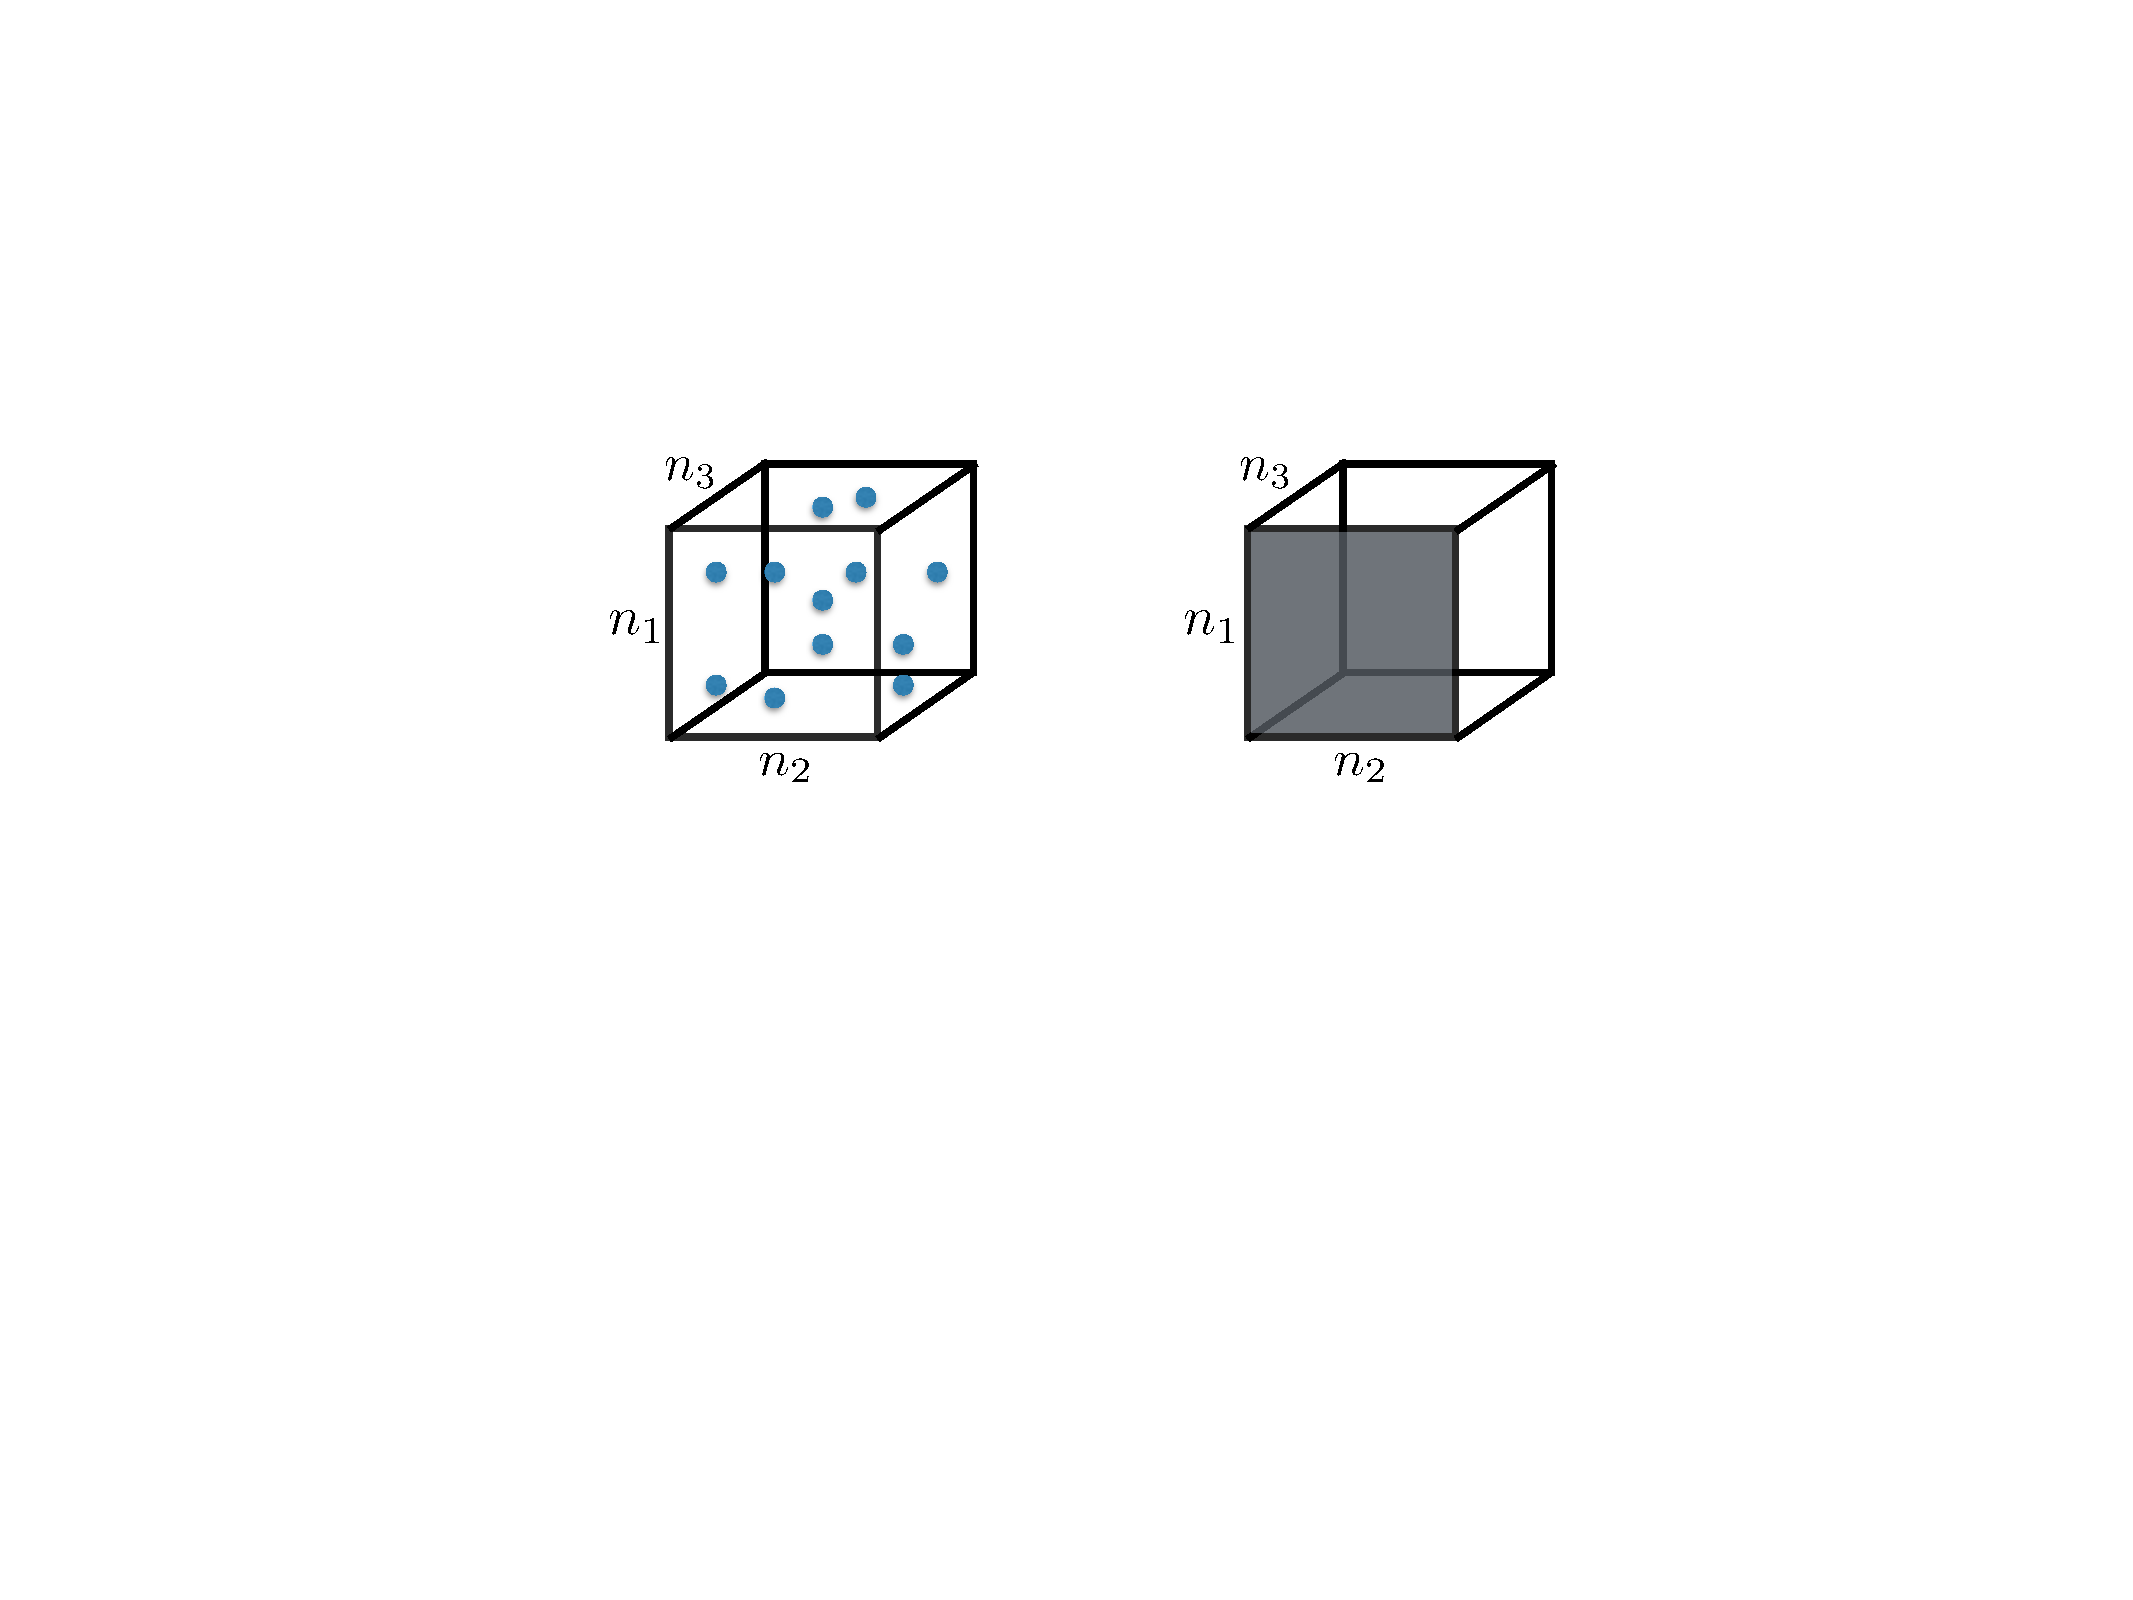
\includegraphics[width=0.6\linewidth]{thpropfigs/sparseanddense}
  \caption{A visualization of an order 3 ($d=3$) sparse and dense tensor (left and right, respectively.}
  \label{fig:sparseanddense}
\end{figure*}
An emerging area of research in computational science considers efficiently computing on data sets that are 
inherently multi-way-- that is, they can be represented by higher-order \emph{tensors}~\cite{Acar09futuredirections}. 
%
% Whereas matrix and block-matrix methods are widespread and well-understood in computational science, a current challenge is to develop \emph{tensor}-level thinking that deals with the unique challenges of tensor data sets~\cite{Acar09futuredirections}. 
%
% Tensor \emph{decompositions} are a leading method for compressing or finding structure within these 
% data sets, and increasing the computational scalability of these decompositions is an open research problem.
Tensor \emph{decompositions} are a powerful tool for the analysis of multi-way data~\cite{Kolda:2009}, and generally attempt to express an input tensor in a form that is lower-dimensional or of a more desirable structure. The resulting decomposition may be valuable for its interpretability (e.g., for factor analysis), or as a compressed format that alleviates the curse of dimensionality. Two of the most popular decompositions are visualized in~\cref{fig:decomps}.
%
% It is tempting to think of tensor computations as inherently more costly than matrix computations.
% A key argument of this proposal however is that the multi-way structure of tensors surprisingly creates numerous avenues for increasing scalability that are not available in the realm of matrix computations.

Because tensor data can scale arbitrarily large (exponential in their order, if each dimension is of a similar size), it is desirable to develop algorithms that scale in kind. We propose to utilize \emph{randomized} methods towards this end.
Recent developments in randomized numerical linear algebra utilize techniques such as random projection and 
sampling to perform common operations such as low-rank 
decomposition and least squares much faster than traditional methods, with the 
drawback that error bounds must often be restated in probabilistic terms. A central motivation in this proposal is the belief that
the dimensionality of tensors lends itself \emph{particularly} well to these randomized methods. 

Towards this goal we propose to develop efficient, high-performance implementations of randomized algorithms for leading tensor decompositions. We demonstrate in our prior work that the \textsc{Candecomp/Parafac} (CP) decomposition can be performed with randomized least squares, and that the tensor structure actually produces favorable conditions for the algorithm-- in fact, the randomized algorithm can extract more robust features than the leading deterministic algorithm at much lower cost~(\cref{sec:cp}). 

In addition we target scaling up the Tucker decomposition in distributed memory using methods drawn from the randomized SVD~(\cref{sec:tucker}), and propose that the tensor structure also suits both this method and another computation, the Tensor Train decomposition~(\cref{sec:tt}). 
%
\begin{figure}
  \centering 
  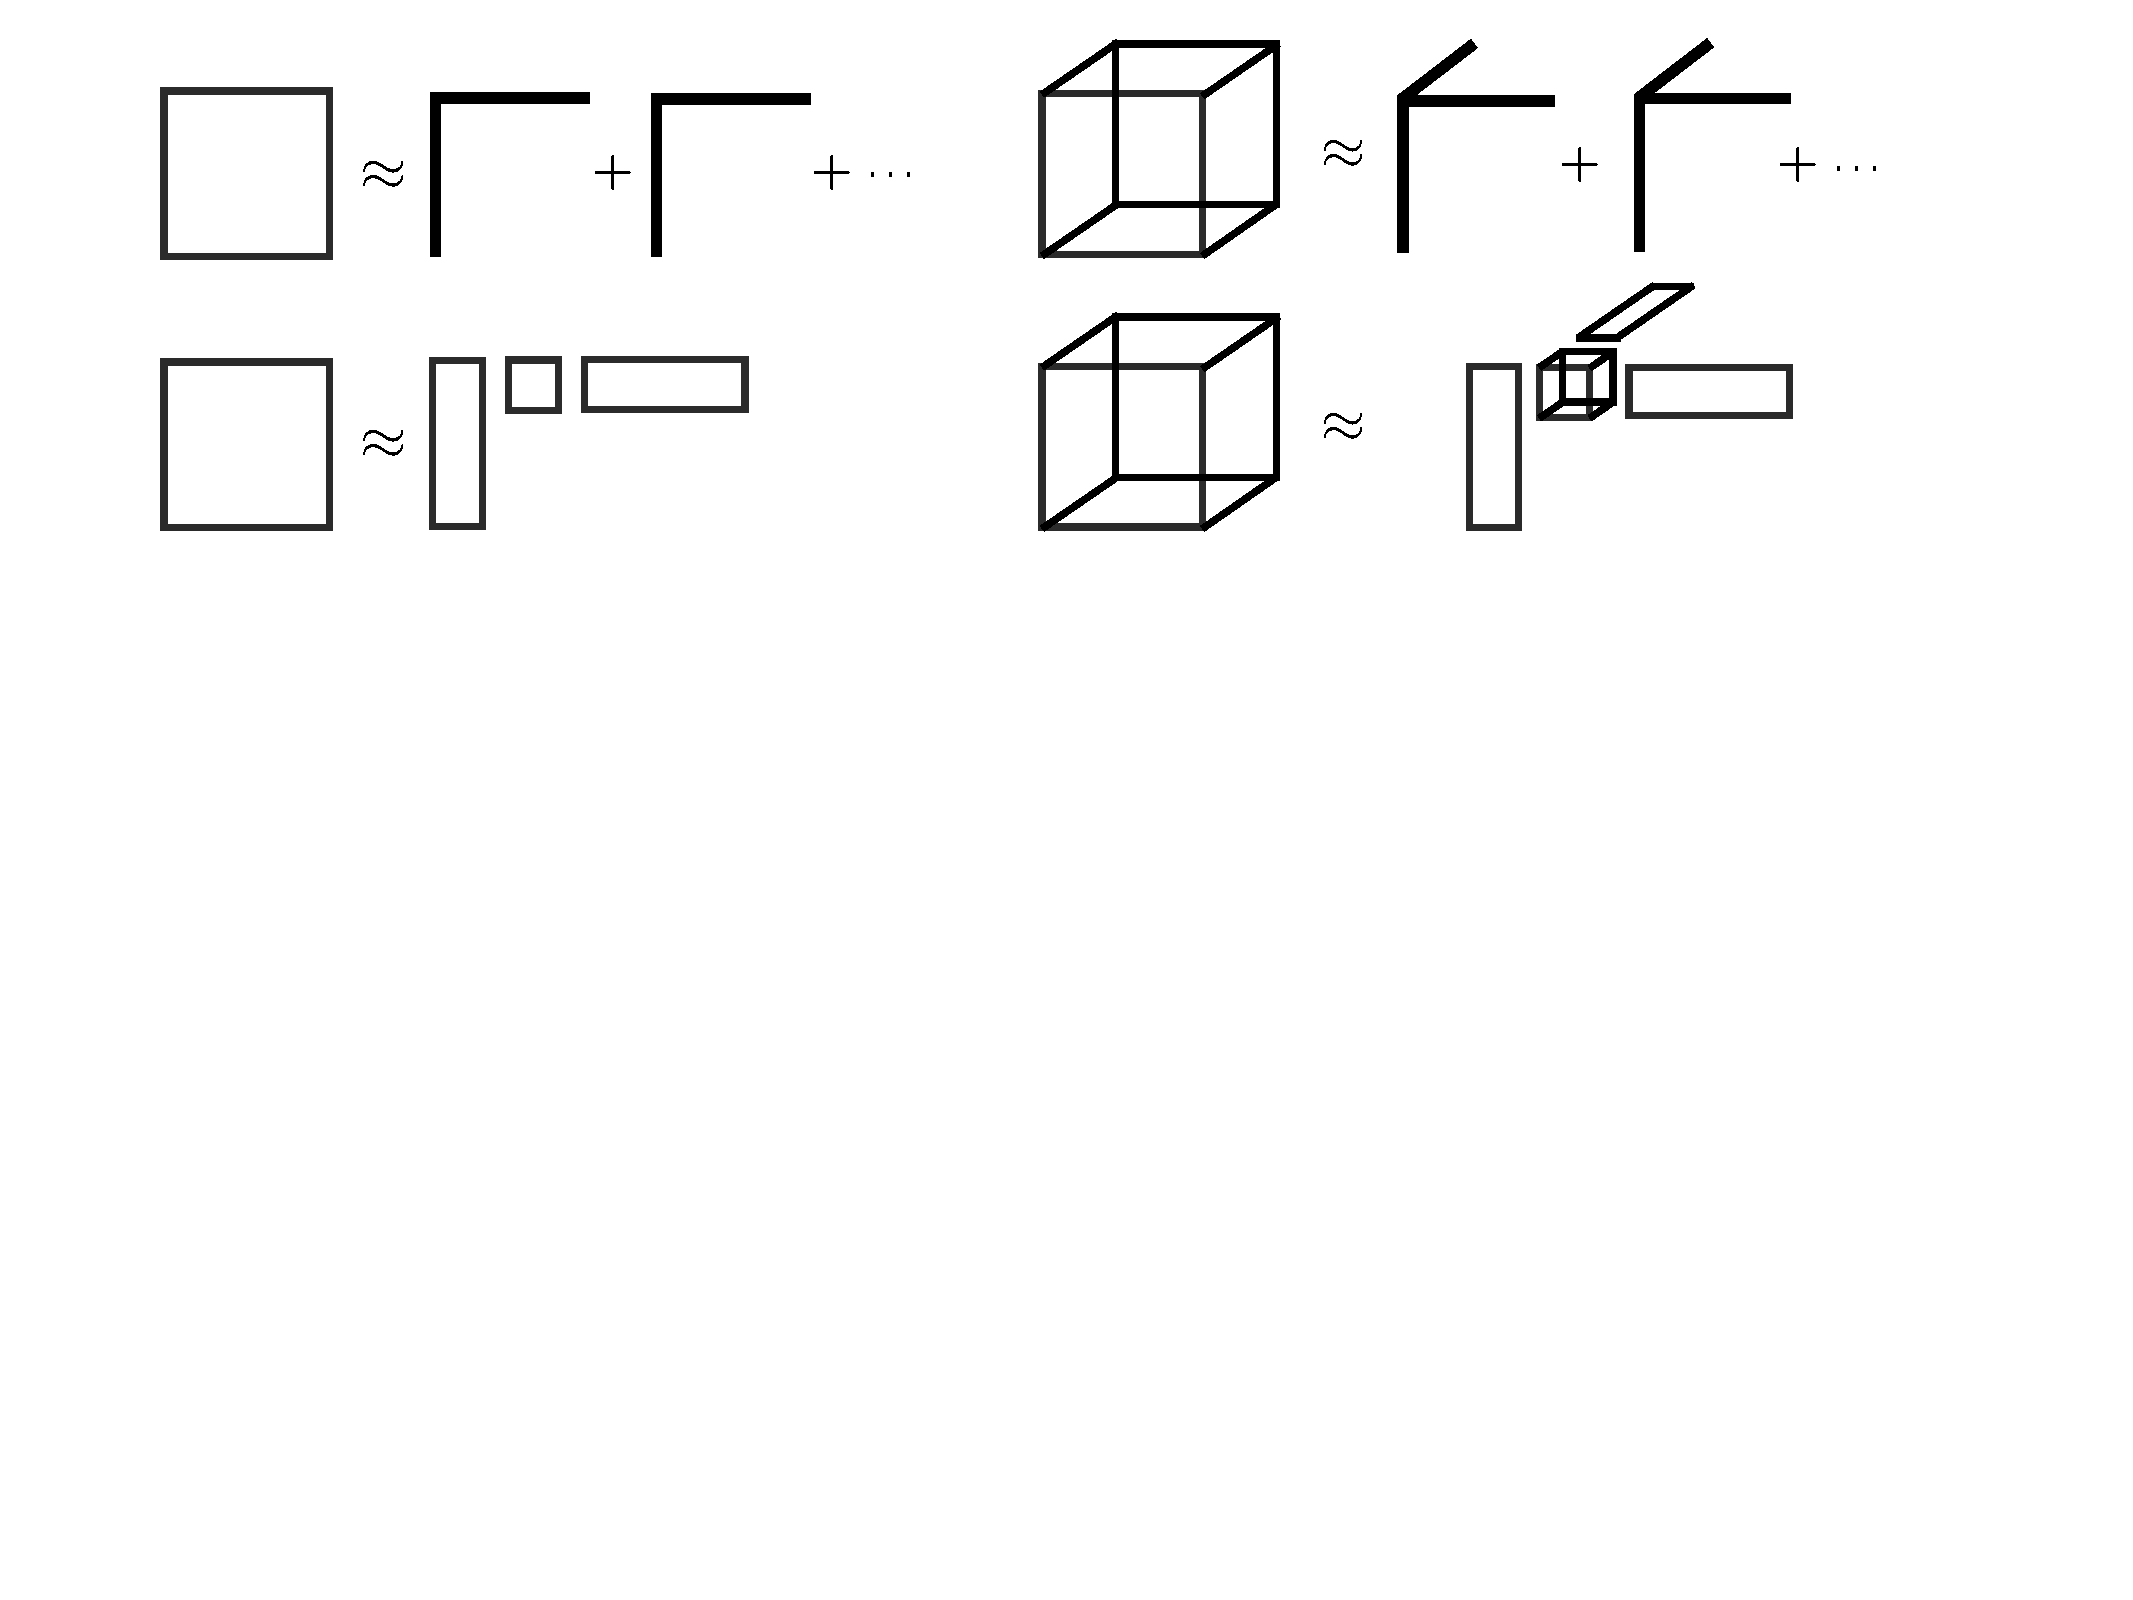
\includegraphics[width=\linewidth]{thpropfigs/decomps}
  \caption{Left: A low-rank matrix decomposition, visualized as a sum of rank-one matrices (top) or as a product of smaller matrices (bottom). Right: The CP decomposition, which is a sum of rank-one tensors (top), and the Tucker decomposition, which is a product of a smaller tensor with $d$ factor matrices in each mode (bottom).}
  \label{fig:decomps}
\end{figure}
%

\subsection{Proposal}
We propose a line of research to apply sketching techniques to tensor decompositions, and to leverage them in such a way that allows for high-performance algorithms that outperform the state of the art. A key aspect within each decomposition is to show how sketching algorithms can leverage the specific higher-order structure of tensors.
\begin{enumerate}
\item \textsc{Candecomp/Parafac} (CP) Decomposition
\begin{itemize}
	\item The leading method for computing the CP decomposition is CP-ALS, which performs iterative least-squares updates in each mode.
	\item In completed work~\cite{caseyb}, we use methods drawn from \emph{randomized least squares} and apply them to this core computation.
	\item We show that the tensor structure produces conditions favorable for sketching.
	\item We also show that tensor dimensionality produces conditions favorable to sampling, which is not necessarily true for matrices.
	\item We demonstrate scalability on real and synthetic data sets.
	\item We demonstrate the surprising result that this method often works \emph{better} than CP-ALS, returning good solutions more robustly.
	\item Deliverable: this method is published~\cite{caseyb} and released as part of MATLAB Tensor Toolbox\footnote{\url{http://gitlab.com/tensors/tensor_toolbox}}~\cite{TTB_Software}.
\end{itemize}
\item Tucker Decomposition / HOSVD
\begin{itemize}
	\item The leading method for computing the Tucker decomposition is the HOSVD, which performs mode-wise SVDs followed by tensor contractions.
	\item We propose to apply ideas from the Randomized SVD to the HOSVD in distributed memory.
	\item We propose that the tensor structure makes random projection highly efficient because it can be expressed as a series of small tensor contractions without intermediate communication. 
	\item We propose that the tensor structure uniquely allows for high-quality output because the efficiency of projections allows for significant \emph{oversampling} in very little time.
	\item We propose to demonstrate scalability on massive real and synthetic data sets on up to 1000 nodes.
	\item Deliverable: this method will be submitted for publication and included as part of TuckerMPI\footnote{\url{http://tensors.gitlab.io/TuckerMPI/}}.
\end{itemize}
\item Tensor Train Decomposition
\begin{itemize}
	\item The tensor train decomposition is a leading low-rank representation for very high-order tensors.
	\item We propose exploring how the structure of the tensor train computation can be exploited by randomized methods in a way comparable to the previous two methods (CP/Tucker).
	\item We propose demonstration of scalability on massive real and synthetic data sets.
	\item We propose developing a practical framework for the tensor train and quantized tensor train that allows for randomization. 
\end{itemize}
\end{enumerate}

\section{Background and Definitions} \label{sec:background} 
% BACKGROUND sec:background %%%%%%%%%%%%%%%%%%%%%%%%%%%%%%%%%%%%%%%%%%%%%%%%%%%%%%%%%%%%%%%%%%
In this section, we provide information on the necessary tensor properties and operations, and then introduce tensor decompositions and associated randomized methods.
%
\subsection{Tensors}
A tensor is an element in a tensor product of vector spaces. In data analysis, 
it suffices to think about a tensor as a multidimensional array.
We represent a tensor as a Euler script capital letter, e.g., 
$\T{X}\in \R^{n_1 \times \cdots \times n_d}$. 

The number of \emph{modes} (or dimensions) of a tensor is referred to as its \emph{order}, 
denoted by $d$. The values $n_k$ denote the dimensions of a tensor, and we let $n=\sqrt[d]{\prod_k n_k}$, 
so that $n^d = \prod_k n_k$. Thus, the term $n^d$ to more intuitively expresses the number of elements 
 in a tensor as exponential in its order. We also let $n_k^\oslash = n^d / n_k$ represent the product of all 
 dimensions \emph{except} $n_k$.

Let $\mathcal{I} = \{ \V{i} = (i_1,\dots,i_d) \}$ be the set of indices of a tensor. 
We can thus express an individual element of a tensor $\T{X}$ for any multiindex $\V{i}$ as $x_{\V{i}}$. 

The \emph{mode-$k$ fibers} of a tensor are higher-order analogues
of matrix columns and rows.
The mode-$k$ \emph{unfolding} or \emph{matricization} of a tensor 
aligns the mode-$k$ fibers as the columns of an $n_k \times n_k^\oslash$ matrix. 
Assuming 1-indexing, tensor entry $x_{\mathbf{i}}$ then maps to
entry $(i_k, j)$ of $\M{X}_{(k)}$ via the relation: 
\begin{equation}
  \label{eqn:unfoldmapping}
  j = 1+\sum_{\substack{\ell=1\\\ell\neq k}}^d (i_\ell -1)m_\ell, \qquad \text{where} \qquad m_\ell = \prod_{\substack{q=1\\q\neq \ell}}^{\ell-1} n_q.
\end{equation}
The \emph{norm} of a tensor is the square root of the sum of its squared entries, 
e.g., $\|\T{X}\| = \|\M{X}_{(k)}\|_F$ for any $k$. Given a decomposed representation $\T{M}$ of a tensor,
the normalized residual error can be written as:
\begin{equation}
\label{eqn:residual}
\|\T{X}-\T{M}\|/{\|\T{X}\|}
\end{equation}
Given matrices $\M{A} \in \mathbb{R}^{n_1 \times n_2}$ and $\M{B} \in \mathbb{R}^{m_1
  \times m_2}$, their \emph{Kronecker product} is 
\begin{displaymath}
  \M{A} \otimes \M{B} =
  \begin{bmatrix}
    a_{11} \M{B} & a_{12} \M{B} & \cdots & a_{1n_2} \M{B} \\
    \vdots & \vdots & \ddots & \vdots \\
    a_{n_1 1} \M{B} & a_{n_1 2} \M{B} & \cdots & a_{n_1 n_2} \M{B} \\
  \end{bmatrix}
  \in \R^{n_1 m_1 \times n_2 m_2}.
\end{displaymath}
%
Assuming $n_2 = m_2$, their \emph{Khatri-Rao product}, also known as the
\emph{matching columnwise Kronecker product}, is
\begin{displaymath}
  \M{A} \odot \M{B} = 
  \begin{bmatrix}
    \V{a}_1 \otimes \V{b}_1 & \V{a}_2 \otimes \V{b}_2
    & \cdots &  \V{a}_J \otimes \V{b}_J \in \mathbb{R}^{n_1 m_1 \times n_2}.   
  \end{bmatrix}
\end{displaymath}
Assuming $n_1=m_1$ and $n_2=m_2$, their \emph{Hadamard product} is
$\M{A}\circledast\M{B} \in \mathbb{R}^{n_1 \times n_2}$, the elementwise product of the matrices.
Three useful identities involving the products just defined are:
\begin{align}
(\M{A} \odot \M{B})^\trans(\M{A} \odot \M{B}) &= \M{A}^\trans\M{A} \circledast \M{B}^\trans\M{B}, \label{eq:KRGram} \\ 
\M{A}\M{B} \otimes \M{C}\M{D} &= (\M{A} \otimes \M{C})(\M{B} \otimes \M{D}) \label{eqn:krondist},\quad\text{and} \\
\M{A}\M{B} \odot \M{C}\M{D} &= (\M{A} \otimes \M{C})(\M{B} \odot \M{D}). \label{eqn:krdist}
\end{align}

%
The \emph{mode-$k$ tensor-times-matrix product} (TTM) is a contraction
between a matrix and a tensor in its $k$th mode.
\begin{equation}
\label{eqn:ttm}
\T{Y} = \T{X} \times_k \M{A} \quad \Leftrightarrow \quad \M{Y}_{(k)} = \M{A}\M{X}_{(k)}.
\end{equation}
We can also write this element-wise as
\begin{equation}
  \label{eqn:contractionelem}
  y_{i_1i_2\cdots i_{k-1}j i_{k+1}\cdots i_d} = \sum_{i_k}x_{i_1\cdots i_d}u_{j i_k}
\end{equation}
We will use bracket notation to denote multiple products, e.g. 
$\T{X} \times \{\Mn{U}{k}\}$ refers to $\T{X}$ multiplied by $\Mn{U}{k}$ 
for every $k=1,\dots,d$. The result is invariant to which order the TTMs are performed in, 
providing the modes are unique. If a tensor can be written as a series of 
mode-$k$ products, its mode-$k$ matricization has a particular structure~\cite{Kolda:2009}:
\begin{align}
  \begin{split}
    \label{eqn:ttensor}\T{Y} & ={}  \T{X} \times \{\Mn{U}{k}\} \quad \Leftrightarrow \\
    \M{Y}_{(k)} & ={}  \Mn{U}{k} \M{X}_{(k)} 
    (\Mn{U}{d} \otimes \cdots \otimes \Mn{U}{k+1} \otimes \Mn{U}{k-1} \otimes \cdots \otimes \Mn{U}{1})^\trans.
  \end{split}
\end{align}
%
\begin{table}[ht]
  \centering\footnotesize
  \label{tab:notation}
  \begin{tabular}{cl}
    \toprule
    Notation & Definition \\
    \midrule
    $\M{X}_{(k)}$ & mode-$k$ unfolding of $\T{X}$ \\
    $\T{X}\times_k \M{U}_k$ & Tensor-Times Matrix Multiplication (TTM) \\
    $\M{A}\otimes\M{B}$ & Kronecker Product \\
    $\M{A}\odot\M{B}$ & Khatri-Rao Product \\
    $\M{A}\circledast \M{B}$ & Hadamard Product \\
    \midrule
    $d$ & Number of modes (order) of a tensor \\
    $n_k$ & Size of mode $k$ of tensor $\T{X}$ \\
    $r_k$ & Rank (core size) of mode $k$\footnote{For the CP decomposition there is only one rank $r$} \\
    $p_k$ & Number of processors along mode $k$ \\
    $s_k$ & Sketch size of mode $k$ \\
    $n,r,p,s$ & $\sqrt[d]{\prod n_k}, \sqrt[d]{\prod r_k}, \sqrt[p]{\prod p_k}, \sqrt[d]{\prod s_k}$ \\
    $n_k^\oslash,r_k^\oslash,p_k^\oslash,s_k^\oslash$ & $n^d/n_k,r^d/r_k,p^d/p_k,s^d/s_k$ \\
    % \midrule
    % $\Mn{U}{k}\in\mathbb{R}^{n_k\times r_k}$ & Tucker factor matrix for mode $k$ \\
    % $\M{\Omega}_k\in\mathbb{R}^{n_k \times s_k}$ & Random sketch matrix for mode $k$ \\
    % $\T{G}\in\mathbb{R}^{r_1\times\cdots\times r_d}$ & Tucker core \\
    % $\T{M} = \{\T{G},\{\M{U}_k\} \}$ & Tucker approximation of $\T{X}$ \\
    % $\bar{\T{X}}$ & Local subtensor of $\T{X}$ \\
    \bottomrule
  \end{tabular}
  \caption{Basic tensor notation used in this proposal.}
\end{table}
%
\subsection{CP Decomposition}
The CP tensor decomposition aims to approximate an order-$d$ tensor as
a sum of $r$ rank-one
tensors~\cite{hitchcock-sum-1927, CANDECOMP, PARAFAC, Kolda:2009}:  
\begin{equation}
\label{eqn:cpform}
\T{X} \approx \T{\tilde{X}} = \sum_{k=1}^d \V{a}_k^{(1)} \circ \V{a}_k^{(2)} \circ \cdots \circ \V{a}_k^{(d)},
\end{equation}
where \emph{factor vector} $\V{a}_r^{(k)}$ has length $n_k$. 
Each rank-one tensor is called a \emph{component}.
The collection of all factor vectors for a given mode is called a 
\emph{factor matrix}:
\begin{displaymath}
  \Mn{A}{k} =
  \begin{bmatrix}
    \MnC{A}{k}{1} &
    \MnC{A}{k}{2} &
    \cdots &
    \MnC{A}{k}{r}
  \end{bmatrix}
  \in\R^{n_k \times r}.
\end{displaymath}
The mode-$k$ matricization of $\T{\tilde{X}}$ can be written in terms
the factor matrices as
\begin{equation}\label{eq:Zn}
  \M{\tilde{X}}_{(k)} = \M{A}^{(k)}\M{Z}^{(k)\trans}
  \qtext{where}
  \M{Z}^{(k)}=\M{A}^{(d)}\odot \cdots  \M{A}^{(k+1)}\odot
  \M{A}^{(k-1)} \odot \cdots \odot \M{A}^{(1)}.   
\end{equation}
We may alternatively represent \cref{eqn:cpform} by normalizing all
the factor vectors to unit length and expressing the product of the
normalization factors as a scalar weight $\lambda_r$ for each
component: 
\begin{equation}\label{eq:cpformlambda}
  \T{\tilde{X}} = \sum_{k=1}^d \lambda_k \; \V{a}_k^{(1)} \circ
  \V{a}_k^{(2)} \circ \cdots \circ \V{a}_k^{(d)}.
\end{equation}

\subsubsection{CP-ALS}

The standard method for fitting the CP model is alternating least
squares (CP-ALS) \cite{PARAFAC,Kolda:2009}. The method alternates
among the modes, fixing every factor matrix but $\Mn{A}{k}$ and
solving for it. From \cref{eq:Zn}, 
we see that we can find $\Mn{A}{k}$ by solving the linear least squares
problem given by
\begin{equation}
\label{eq:lls}
\argmin_{\M{A}^{(k)}} \|\M{X}_{(k)} - \M{A}^{(k)}\M{Z}^{(k)\trans}\|_F.
\end{equation}
In CP-ALS, we work with the normal equations for \cref{eq:lls}:
\begin{displaymath}
\M{X}_{(k)}\M{Z}^{(k)} = \M{A}^{(k)}(\M{Z}^{(k)\trans}\M{Z}^{(k)}),
\end{displaymath}
and solve for $\M{A}^{(k)}$ for given $\M{X}_{(k)}$ and $\M{Z}^{(k)}$.
By identity \cref{eq:KRGram}, we have 
\begin{equation}
\label{eqn:nicegram}
\M{Z}^{(k)\trans}\M{Z}^{(k)} = \M{A}^{(d)\trans}\M{A}^{(d)} \circledast \dots \circledast \M{A}^{(k+1)\trans}\M{A}^{(k+1)} \circledast \M{A}^{(k-1)\trans}\M{A}^{(k-1)} \circledast \cdots \circledast \M{A}^{(1)\trans}\M{A}^{(1)}.
\end{equation}

The CP-ALS algorithm~\cite{Kolda:2009} is presented
in~\cref{alg:cpals}. Note the step where vector $\bm{\lambda}$ stores
normalization values of each column so that the final approximation is
as in \cref{eq:cpformlambda}; this normalization helps alleviate
issues due to scaling ambiguity.

The initialization of the factor matrices
can impact the performance of the algorithm.
There are many possible ways to do the the initialization.
One way is to
initialize is to set $\Mn{A}{k}$ to be the leading $r$ left singular
vectors of the mode-$k$ unfolding, $\M{X}_{(k)}$, and we call this
HOSVD initialization, as it corresponds to the factor matrices
in the rank-$(r{\times} {\cdots} {\times} r)$ HOSVD (see~\cref{sec:hosvd}). 
A less expensive but less effective initialization is to
choose random factor matrices.

Finally, a termination criterion must be supplied. For instance, a simple way to check convergence is to see when the change in residual error~(\cref{eqn:residual}) becomes negligible.

\begin{algorithm}
  \caption{CP-ALS}
  \label{alg:cpals}
  \begin{algorithmic}[1]\footnotesize
    \Function{$[\bm{\lambda},\set{\M{A}^{(k)}}]=$ CP-ALS}{$\T{X},r$}\Comment{$\T{X}\in\mathbb{R}^{n_1\times \cdots \times n_d}$}
    \State \label{line:cpals:init} Initialize factor matrices $\M{A}^{(2)}, \dots, \M{A}^{(d)}$
    \Repeat
    \For{$k=1,\dots, d$}
      \State $\M{V} \gets \M{A}^{(d)\trans}\M{A}^{(d)} \circledast \dots \circledast \M{A}^{(k+1)\trans}\M{A}^{(k+1)} \circledast \M{A}^{(k-1)\trans}\M{A}^{(k-1)} \circledast \cdots \circledast \M{A}^{(1)\trans}\M{A}^{(1)}$\label{line:cpals:Gram}
      \State \label{line:cpals:KR} $\M{Z}^{(k)} \gets \M{A}^{(d)}\odot \cdots  \odot \M{A}^{(k+1)}\odot \M{A}^{(k-1)} \odot \cdots \odot \M{A}^{(1)}$
      \State \label{line:cpals:MTTKRP} $\M{W} \gets \M{X}_{(k)}\M{Z}^{(k)}$
      \State \label{line:cpals:solve} Solve $\M{A}^{(k)}\M{V} = \M{W}$ for $\M{A}^{(k)}$        
      \State Normalize columns of $\M{A}^{(k)}$ and update $\bm{\lambda}$
    \EndFor
    \Until termination criteria met
    \State \textbf{return} $\bm{\lambda}$, factor matrices $\set{\M{A}^{(k)}}$
    \EndFunction
  \end{algorithmic}
\end{algorithm}

Because of the elegant least squares structure in~\cref{eqn:nicegram}, the bottleneck for CP-ALS is generally in performing lines 6-7, which we refer to as the matricized Khatri-Rao product (MTTKRP). High-performance implementations of CP-ALS generally target the MTTKRP~\cite{SPLATT,dimtree,koby}. 


\subsection{The Tucker Decomposition} \label{sec:hosvd} 
\begin{figure}[htbp]
  \centering
\begin{tikzpicture}[scale=0.5,namenode/.style={scale=.75}]
	\def\ix{3} %
	\def\iy{3} %
	\def\iz{2.5} %
	\def\corescale{1.75}
	\def\rx{\ix/\corescale}
	\def\ry{\iy/\corescale}
	\def\rz{\iz/\corescale}
	\coordinate (XFrontLowerLeft) at (0,0);
	\draw (XFrontLowerLeft) rectangle ++ (\ix,\iy); %
	\begin{scope}[shift={(XFrontLowerLeft)},canvas is zx plane at y=\iy,rotate=90]
	  \draw (0,0) rectangle ++ (\ix,\iz); %
	\end{scope}
	\begin{scope}[shift={(XFrontLowerLeft)},canvas is zy plane at x=\ix,rotate=90]
	  \draw (0,0) rectangle ++ (\iy,\iz); %
	\end{scope}
	\node[namenode] at ($(XFrontLowerLeft) + (0.5*\ix, 0.5*\iy)$)  {$\T{X}$};
	\coordinate (ApproxCtr) at ($(XFrontLowerLeft) + (\ix+0.4*\iz,0.75*\iy) + (0.75,0)$);

	\node[namenode] at (ApproxCtr) {$\approx$};
	\coordinate (U1LowerLeft) at ($(ApproxCtr) - (0,0.75*\iy) + (0.75,0)$);
	\draw (U1LowerLeft) rectangle ++ (\ry,\iy);

	\node[namenode] at ($(U1LowerLeft)+(0.5*\ry, 0.5*\iy)$)  {$\Mn{U}{1}$};
	\coordinate (GFrontLowerLeft) at ($(U1LowerLeft) + (\ry+0.5,1)$);
	\draw (GFrontLowerLeft) rectangle ++ (\rx,\ry);
	\begin{scope}[shift={(GFrontLowerLeft)},canvas is zx plane at y=\ry,rotate=90]
	  \draw (0,0) rectangle ++ (\rx,\rz);
	\end{scope}
	\begin{scope}[shift={(GFrontLowerLeft)},canvas is zy plane at x=\rx,rotate=90]
	  \draw (0,0) rectangle ++ (\ry,\rz);
	\end{scope}
	\node[namenode] at ($(GFrontLowerLeft)+(0.5*\rx,.5*\ry)$)  {$\T{G}$};
	\coordinate (U2LowerLeft) at ($(GFrontLowerLeft) + (\rx+\rz*0.4+0.5,0.5)$);
	\draw (U2LowerLeft) rectangle ++ (\ix,\rx); %

	\node[namenode] at ($(U2LowerLeft)+(0.5*\ix,0.5*\rx)$)  {$\Mn{U}{2}$};
	\coordinate (U3LowerLeft) at ($(GFrontLowerLeft) + (0.5,\ry+.8)$);
	\begin{scope}[shift={(U3LowerLeft)},canvas is zx plane at y=0,rotate=90]
	  \draw (0,0) rectangle ++ (\rz,\iz); %
	\end{scope}
	\node[namenode] at ($(U3LowerLeft)+(1.2,0.5)$) {$\Mn{U}{3}$};
\end{tikzpicture}
  \caption{Tucker decomposition of 3rd-order tensor ($d=3$).}
  \label{fig:thirdordertucker}
\end{figure}
%%% Local Variables:
%%% mode: latex
%%% TeX-master: t
%%% End:
 %%%%%% Tucker Figure %%%%%%
The Tucker decomposition~\cite{Tu66} approximates a tensor with a core tensor contracted with 
matrices in each mode:
\begin{displaymath}
  \T{X} \approx \T{M} = \T{G} \times_1 \Mn{U}{1} \times_2 \Mn{U}{2} \cdots \times_d \Mn{U}{d} = \T{G} \times \{\Mn{U}{k}\},
\end{displaymath}
where
$\T{G}$ is a dense core of size $r_1 \times r_2 \times \cdots \times r_d$, and the factor matrices 
$\Mn{U}{k}$ have size $n_k \times r_k$ for $k=1, \dots, d$.

The \hosvd~\cite{Lathauwer00amultilinear} is a method for computing the Tucker decomposition that computes a series 
of SVDs of
unfolded tensors to compute the orthogonal factor matrices $\Mn{U}{k}$ whose 
columns approximately span the columns of the unfolded tensor $\M{X}_{(k)}$ for each mode $k$. We will refer to this computation as the Mode-wise Truncated Fiber Space Basis Computation (\MTFSBC).
Following this operation, the resulting factor matrices are applied to the input tensor to compress the original data into the core $\T{G}$: $\T{G} \gets \T{X} \times \{ \Mn{U}{k}^\trans \}$. 

Just as we would compress a matrix by truncating its SVD, we can truncate the factors 
$\Mn{U}{k}$ so that $\T{G}$ is a smaller core ($r_k < n_k$), a method we refer to as the 
\emph{truncated} \hosvd (\thosvd), presented in~\cref{alg:sthosvd}.
This is particularly effective for compression; as with $n$, we let $r=\sqrt[d]{\prod r_k}$, and so 
the core is exponentially smaller than $\T{X}$, a factor of $(\frac{n}{r})^d$. 
The total compression ratio includes the factor matrices:
\begin{equation}
\label{eqn:compression}
n^d / \left(r^d + \sum_{k=1}^d n_k r_k\right).
\end{equation}

The HOSVD can be
implemented by forming the $n_k \times n_k$ Gram matrix $\M{S}_k = \M{X}_{(k)}\M{X}_{(k)}^\trans$ 
and computing its eigendecomposition. The eigenvectors of $\M{S}_k$ correspond to the left
singular vectors of $\M{X}_{(k)}$, and $\lambda_j(\M{S}_k) = \sigma_j(\M{X}_{(k)})^2$. 
This Gram computation is utilized by TuckerMPI, which performs a distributed Gram matrix 
computation followed by a local eigendecomposition~\cite{AuBaKo16}.
We use the Gram variant because we 
assume that dimensions are reasonably-sized, e.g., $n_k \leq 10^4$ for all $k$.

\begin{algorithm}[htb]
  \caption{\thosvd\Comment{Gram Variant}}
  \begin{algorithmic}[1]
    \Procedure{\thosvd}{$\T{X}$, $(r_1,\dots,r_d)$}
    \For{$k=1,\dots,d$}
    % \State $[\M{U},\M{\Sigma}] \gets \text{SVD}(\M{X}_{(k)})$
    \State $\M{S}_k \gets \M{X}_{(k)}\M{X}_{(k)}^\trans $ \Comment{Gram}
    \State $[\M{U},\M{\lambda}] \gets \text{eig}(\M{S}_k)$ \Comment{Eigensolve}
    % \State $r_k \gets $ min $j$ s.t. $\sum_{r>j} \lambda_r \leq \epsilon^2\|\T{X}\|^2/d$
    \State \label{line:sthosvd:svd} $\Mn{U}{k} \gets \text{ leading $r_k$ eigenvectors in $\M{U}$}$
    \EndFor
    \State \label{line:sthosvd:trunc} $\T{G} \gets \{ \T{X} \times \Mn{U}{k}^\trans\}$ \Comment{TTM (Core Formation)}
    \State $\T{M} \gets \{ \T{G}, \set{\Mn{U}{k}} \}$ \label{line:sthosvd:ttm}
    \State \Return $\T{M}$
    \EndProcedure
  \end{algorithmic}
  \label{alg:sthosvd}
\end{algorithm}
%
A new variant of the \thosvd is the \emph{sequentially} truncated \hosvd (\sthosvd)~\cite{sthosvd}, 
which is implemented in TuckerMPI~\cite{AuBaKo16}. Whereas the \thosvd forms the core 
after performing the \MTFSBC for all modes (in~\cref{line:sthosvd:ttm}), 
the \sthosvd performs a \MTFSBC for a single mode followed by a core-compression step in that mode,
such that the $k$th TTM occurs within the $k$th iteration of the for loop. 
The working size of the tensor thus reduces by a 
factor of $n_k / r_k$ at each iteration, with an equivalent reduction in the cost of subsequent SVD steps.
%



\subsection{Tensor Train Decomposition}
The Tensor Train decomposition (TT) factors an order-$d$ tensor into a set of $d$ tensors. The $k$th tensor is denoted $\T{G}^{(k)}$, where $\M{G}^{(1)}$ and $\M{G}^{(d)}$ are of order 2 (matrices), and all other tensors are of order 3. 

The input tensor can then be reconstructed via the relation:
\begin{equation}
\T{X} \approx \M{G}^{(1)} \times_{2}^1 \T{G}^{(2)} \times_{3}^1 \T{G}^{(3)} \times_3^1 \dots
\times_3^1 \T{G}^{(d-1)}\times_3^1 \M{G}^{(d)} 
\end{equation}
where $\T{X} \times_a^b \T{Y}$ can be computed as a reordering (`tensorization') of $\M{Y}_{(b)} \M{X}_{(a)}$, or more generally as 
\begin{align*}
\T{X}(i_1,\dots,i_d) & \approx  
\sum_{{k_1}=1}^{r_1} \sum_{{k_2}=1}^{r_2}\cdots\sum_{{k_{d-1}}=1}^{r_{d-1}} \M{G}^{(1)}(i_1,k_1)\T{G}^{(2)}(k_1,i_2,k_2) & \\ & \cdots\T{G}^{(d-1)}(k_{d-2},i_{d-1},k_{d-1})\M{G}^{(d)}(k_{d-1},i_d)
\end{align*}
where $\M{G}^{(1)}\in \R^{r_1\times n_1}$, $\T{G}^{(k)} \in \R^{r_{k-1}\times n_k \times r_k}$ for $1< k< d$ and $\M{G}^{(d)}\in \R^{R_{d-1}\times n_d}$. The relationship between tensors can be better understood in terms of a tensor network diagram. In this visualization, each node represents a tensor, and each line represents a mode, with the associated mode size. Lines that connect tensors represent the common mode that can be contracted to reconstruct the input tensor:
\begin{figure}[htbp]
    \center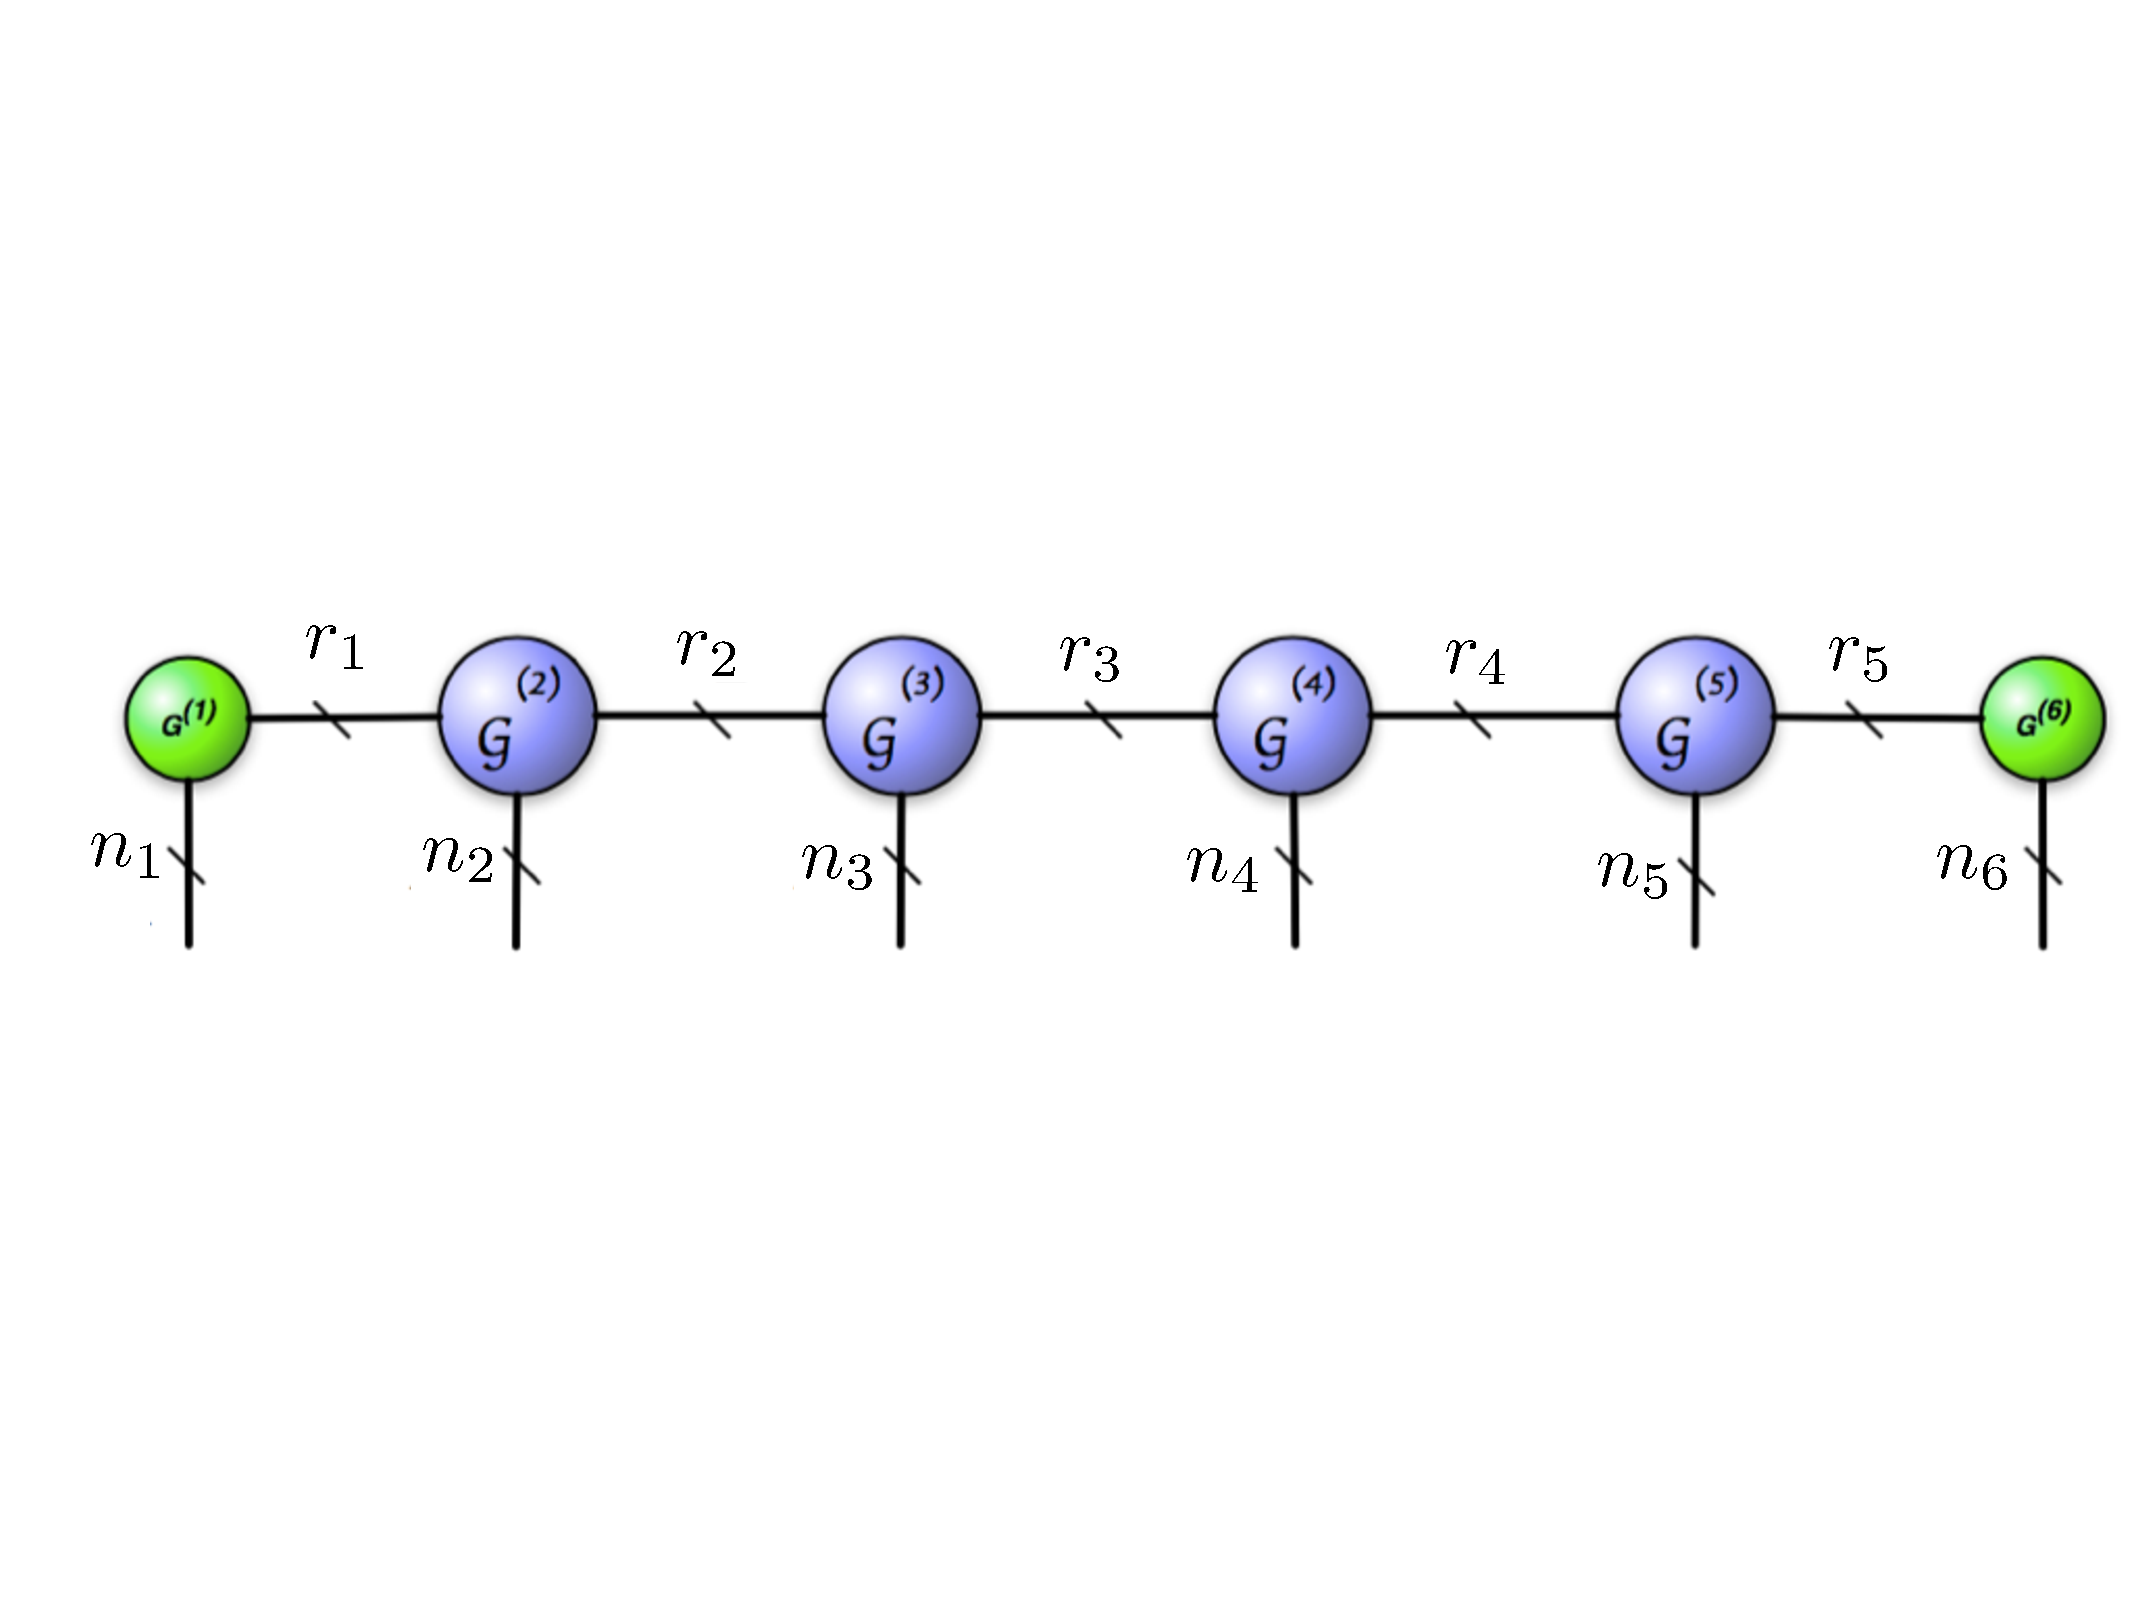
\includegraphics[width=0.80\linewidth]{thpropfigs/tensortrain}
    \caption{Tensor Train Decomposition}
\end{figure}
The most straightforward way to compute a tensor train decomposition is to flatten the tensor and compute a rank-revealing matrix decomposition of the result. The left factor of this decomposition becomes a new node in the tensor train, while the remaining product is reshaped and used as an input for further iterations. 

Tensor network representations such as the tensor train are particularly valuable in cases where the order of a tensor is so high that the dense core of the Tucker decomposition is not feasible to construct. Among many applications it has proven useful in deep learning~\cite{ttrnn,ttnn}, supervised learning~\cite{supervisedtt}, and control systems~\cite{ttcontrol}. It has also proven useful for the approximation of functions~\cite{GoKaMa15}.

\subsection{Randomized Least Squares}
\label{sec:sketching}
Sketching is a technique for solving linear algebra problems by constructing 
a smaller problem whose solution is a 
reasonable approximation to the original problem with high probability~\cite{sketching}. 
For instance, a large matrix may be formed by applying random sampling or random 
projections to form a smaller \emph{sketch} matrix. 
We focus on the case where a regression
problem $\min_{\V{x}}\| \M{A}\V{x} - \V{b} \|_2$ (with overdetermined
$\M{A} \in \mathbb{R}^{n\times d}$) is transformed using some random
projection $\M{M} \in \mathbb{R}^{\samplesize\times n}$, with $\samplesize\ll
n$, such that an exact solution to $\min_{\V{x}}\| \M{M}\M{A}\V{x} -
\M{M}\V{b} \|_2$ is an approximate solution to the original
problem~\cite{rokhlintygert,DrMaMuSa11,blendenpik}.


There are two leading sampling approaches for randomized least squares
problems. One involves sampling from the coefficient matrix in a
weighted manner, e.g. by computing (or estimating) \emph{leverage
  scores} for each row and sampling based on their distribution. The
other approach, which we have implemented, is to \emph{mix} the
coefficient matrix with the intention of evenly distributing leverage scores
across all rows in such a way that \emph{uniform} sampling is
effective. 
\begin{definition}
Given $\M{A} \in \mathbb{R}^{n\times d}, n > d$, the \emph{leverage score} of row $i$ of $\M{A}$ is $l_i = ||\M{U}(i,:)||_2^2$
for $i \in \{1,\dots ,n\}$ where $\M{U}$ contains the $d$ left singular vectors of $\M{A}$.
\end{definition}
Thus, the leverage score of a row corresponds in some sense to the
importance of that row in constructing the column-space of the
coefficient matrix. 

In 2007, Drineas et al.~\cite{DrMaMuSa11} presented a relative-error
least squares algorithm that gives a $1 + \epsilon$
approximation. They first mix the coefficient matrix using a
randomized Hadamard transform (discussed later), and then sample 
\begin{equation}
\label{eqn:numsamples}
\bigO{\max\{ d\log{(n)}\log{(d\log{(n)})}, d\log{(nd)}/\epsilon\}}
\end{equation}
rows of the resulting matrix before computing the solution using
normal equations. The dependence of the sampling size on $\epsilon$
makes this algorithm fairly impractical for typical direct
solvers. However, subsequent work by Rokhlin and
Tygert~\cite{rokhlintygert} applied a related sketching strategy to
the \emph{preconditioning} of a Krylov-subspace method, establishing a
relationship between sample size and condition number.  

Avron et al.\@ synthesized these concepts into a high-performance
solver called Blendenpik~\cite{blendenpik}. They first apply a
randomized Hadamard transform (or similar transform),
compute a QR decomposition of the result, and use its
$\M{R}$ factor as a preconditioner
for the standard LSQR solver. Additionally they show that the
condition number of their system depends on the \emph{maximal}
leverage score of the matrix, referred to as \emph{coherence}. 
\begin{definition}[\cite{coherence,candesrecht}]
\emph{Coherence} is  the maximum leverage score of $\M{A}$, i.e.,
\[ \mu(\M{A}) = \max_{i \in \{1,\dots,n\}} l_i, \]
where $l_i$ is the leverage score of the $i$th row of $\M{A}$. It
holds that $\frac{d}{n} \leq \mu(\M{A}) \leq 1$. 
\end{definition}
Intuitively, if a row of a matrix $\M{A}$ contains the only nonzero in a column then $\mu(\M{A})=1$ and any row-sampling $\M{SA}$ must include that row (which has leverage score 1) or it will be rank deficient. If coherence is close to 1, a uniform row-sampling is likely to be \emph{nearly} rank-deficient, leading to a poorly conditioned reduced-size least squares problem and an inaccurate approximate solution vector. 

In~\cite{caseyb} we show that the standard formulation of CP-ALS
may increase incoherence, making uniform sampling effective in many
situations. However, in order to guarantee incoherence (w.h.p.)
regardless of input, it is necessary to preprocess with a mixing step.  

This mixing strategy relates to a more general class of
transformations that rely on quality guarantees provided by the
Johnson-Lindenstrauss Lemma~\cite{jlt}. This lemma specifies a class
of random projections that preserve the distances between all pairs of
vectors with reasonable accuracy. The \emph{fast}
Johnson-Lindenstrauss transform (FJLT) is able to avoid explicit
matrix multiplications by utilizing efficient algorithms such as the
fast Fourier transform (FFT), discrete cosine transform (DCT), or
Walsh-Hadamard Transform (WHT)~\cite{fjlt}. These transforms can
operate on a vector $\V{x} \in \mathbb{R}^n$ in $\inlineBigO{n\log_2 n}$
time. What these algorithms have in common is that
they improve incoherence, mixing information across every element of a vector, while at the
same time being orthogonal operations (i.e., a change of basis).  
The theoretical quality guarantees and theoretical computational costs are the same for all fast transforms.

The FJLT consists of three steps. First, each row of the coefficient
matrix is sign-flipped with probability $1/2$. This is equivalent to
computing $\M{D}\M{A}$ with diagonal matrix $\M{D}\in
\mathbb{R}^{n\times n}$, where each diagonal element is $\pm 1$ with
equal probability. Second, we apply the fast mixing operation
$\mathcal{F}$. Third we uniformly sample $\samplesize$ rows of the
result with uniform probability. Thus, the entire operation can be
written out as $\M{S}\mathcal{F}\M{D}\M{A}$, where $\M{S}$ is a row-sampling operator (containing unit row vectors $\V{e}_{i}$, for each sampled row $i$).
The reasoning behind first
applying $\M{D}$ is that input data is often sparse in the frequency
domain, and randomly flipping the signs of the coefficient matrix is an
orthogonal operation that spreads out the frequency domain of
the signal~\cite{fjlt}. 
% In this paper we will exclusively use the FFT
% for the $\mathcal{F}$ operation due to its ease of reproducibility and its efficiency in
% MATLAB. 
% Though portable, this has the result of making all data complex-valued, which we discuss~\cite{caseyb}.
% We observed that using alternative transforms had no effect on the quality of our solutions, but real-valued transforms were slower to apply because of a lack of efficient implementations within MATLAB.
%
\subsection{Randomized SVD}
The \MTFSBC requires finding the leading left singular vectors and singular values of the tensor 
matricization. Halko, Martinsson, and Tropp ~\cite[Alg.~4.1]{halko} present a \emph{randomized range finder} algorithm 
for estimating the left singular vectors of a matrix $\M{X}$ of size $m \times n$ where $n$ is very large.
The goal is to find the leading $r$ left singular values where it is assumed that the remaining singular values are small.
The key idea is to multiply $\M{X}$ on the right
by a sketching matrix $\M{\Omega}$ of size $n \times q$ where $r < q \ll n$.
The matrix $\M{\Omega}$ is some appropriate random matrix;
for instance, it could have i.i.d.\@ entries drawn from a standard normal distribution.
The result of the multiplication is a much smaller matrix of size $m \times q$ whose $q$ leading left singular vectors approximately include the range of the $r$ leading left singular vectors of $\M{X}$.
The value of $q-r$ is the \emph{oversampling parameter}, and the is typically small, e.g., less than 20.
We summarize the method in \cref{alg:RRF}, and its expected error is analyzed in~\cite{halko}.

\begin{algorithm}[htb]
  \caption{Randomized Range-Finder}\label{alg:RRF}
  \begin{algorithmic}[1]
    \Procedure{RRF}{$\M{X}$, $q$} \Comment{$\M{X} \in \mathbb{R}^{m \times  n}$}
    \State $\M{\Omega} \gets$ suitable random matrix of size ${n \times q}$ 
    \State $\M{Y} \gets \M{X}\M{\Omega}$
    \State \label{line:rrf:ortho} $\M{U} \gets$ orthonormal basis of size $m \times q$ for $(\M{Y})$
    \EndProcedure
  \end{algorithmic}
  \label{alg:rrf}
\end{algorithm}

For this method to be efficient, the desired rank should be small, i.e., $r \ll n$.
If $m \ll n$, then we know that $r \leq m \ll n$, so this property is satisfied. Indeed, we will observe that the matrix
unfoldings in the \MTFSBC have exactly that property since we are working with matrices of roughly 
$n \times n^{d-1}$ in size. 

Sketching methods of this nature have become popular within matrix decompositions~\cite{tropp2}, but have only recently seen use in tensor methods or distributed computation. 
%
\section{Literature Survey}
A broad survey of tensor decompositions is provided by Kolda and Bader~\cite{Kolda:2009}. Additional papers outline specific tensor techniques in machine learning~\cite{nikossurvey}, quantum chemistry~\cite{quantumsurvey}, latent variable models~\cite{Anandk}, and neuroscience~\cite{eegsurvey}. In this proposal we focus on scalable implementations of three of the most popular tensor decompositions: the \textsc{Candecomp/Parafac} (CP) decomposition~\cite{hitchcock-sum-1927, CANDECOMP, PARAFAC}, the Tucker decomposition~\cite{Tu66}, and the Tensor Train decomposition~\cite{tensortrain}. 

\paragraph{Scalable CP Decompositions}
There are many methods that improve performance of the CP decomposition by finding efficient ways of computing MTTKRP kernel within CP-ALS~\cite{SPLATT,dimtree,koby,jiajia2}. Since we propose randomized methods that actually reduce flop count, we survey those methods in more detail:

Vervliet and Lauthauwer present a stochastic gradient descent (SGD) algorithm for CP that samples blocks from the original tensor to update corresponding blocks of the factor matrices~\cite{VeLa16}. This approach is similar in spirit to CPRAND, but takes an altogether different approach to the randomization. They use \emph{contiguous} samples in the block updates and finer control over step sizes. They also update only a portion of each factor matrix in each iteration.

Another framework that draws from SGD is FlexiFaCT, which targets coupled tensor decompositions for parallel computation~\cite{flexifact}

Cheng et al.~have recently applied a leverage score-based sampling to the least-squares step of the sparse CP decomposition by showing how leverage scores of an unfolded tensor can be estimated by the leverage scores of the factor matrices~\cite{spals}. This approach is similar to the way that we bound the coherence of Khatri-Rao products. 
Reynolds et al.~also use randomization within CP-ALS, specifically for the case of rank reduction, where the input to the algorithm is already in CP format \cite{RDB16}.

Wang et al.~have applied sketching methods to \emph{orthogonal} tensors with provable guarantees~\cite{anand}. Song et al.~show that this sketch can be computed without reading the entire tensor (in sublinear time) under certain conditions~\cite{sublinear}.

An alternative to sketching is to compress the tensor using lossy methods before computation. Zhou and Cichocki examine the effectiveness of performing a CP decomposition on a compressed representation of the data using the lossy Tucker decomposition to produce a smaller problem size~\cite{bigtens}. ParCube~\cite{parcube} compresses the original tensor by directly sampling and performs a decomposition on the result.
Another useful approach for high-order tensors is known as tensor reshaping, that can cast much of the computation in terms of three-way tensors \cite{PTC13b}.

\paragraph{Scalable Tucker Decompositions}
The current state of the art for the distributed, deterministic dense \hosvd is TuckerMPI, based on the work of Austin, Ballard, and Kolda~\cite{AuBaKo16}, whereas Kaya and Ucar have optimized the Tucker decomposition in distributed memory for sparse tensors~\cite{kaya1}. In shared memory, optimizations have targeted the core formation step~\cite{intensli}, or developing compressed data structures~\cite{shadentucker}.  

Zhou, Cichocki, and Xie have previously implemented an HOSVD based on the Randomized Ranger Finder algorithm~\cite{bigtens}. They implement RandTucker, which performs a Randomized Range Finder on the \emph{full} matricizations of the tensor, and RandTucker2i, which performs a second iteration after projecting with the first set of estimated factor matrices. 

Vervliet, Debals, and De Lauthawer similarly implement a randomized Tucker in their serial MATLAB toolbox TensorLab3\cite{DBLP:conf/acssc/VervlietDL16}. This allows the user to perform an arbitrary number of iterations that improve the final result. Navasca and Pompey~\cite{Navasca2015} also present a serial HOSVD implementation that uses the randomized SVD on the matricizations in each mode, but it does not take any optimizations into account. Other randomized methods for computing the HOSVD have focused on sampling directly from the tensor~\cite{Tsou10,DM07}.

Our proposed work differs from earlier approaches~\cite{bigtens,DBLP:conf/acssc/VervlietDL16,Navasca2015} in that we target a distributed-memory implementation that performs sketching as a series of small TTMs (equivalent to a Kronecker product of sketching matrices). We also propose to target optimization of the communication involved in this sketching step. 

\paragraph{Scalable Tensor Train Decompositions}
There is not much literature specifically on high-performance tensor train decompositions, so it is a valuable area for future work. Phan, et al. have compared various methods~\cite{Phan2016TensorNF}, but in general the emphasis has been placed on algorithms that operate efficiently by \emph{using} a tensor train representation~\cite{cichocki2}. 

Randomization has been applied to the Tensor Train decomposition in existing work~\cite{HSW17}, but the emphasis has not been on performance. There is also no existing distributed implementation of these methods. Finally, a related tensor network decomposition, the Hierarchical Tucker decomposition, has been successfully targeted with sampling methods~\cite{SHT}.


% \section{Literature Review}

\section{Randomized CP Decomposition} \label{sec:cp} 
The CANDECOMP/PARAFAC (CP) tensor decomposition is an important tool
for data analysis in applications such as chemometrics~\cite{MuStGrBr13}, biogeochemistry~\cite{JaCaYa14},
neuroscience~\cite{AcBiBiBr07,DaGiCaWa13,CoLiKuGo15}, cyber traffic analysis~\cite{MaGuFa11}, and many others.
%
We consider the problem of accelerating the alternating least squares (CP-ALS) algorithm using randomization.

Because randomized methods have been used successfully for solving
linear least squares problems~\cite{DrMaMuSa11,blendenpik,sketching}, it is natural that they might prove
beneficial to CP-ALS since its key kernel is the solution of a least
squares problem. However, the CP-ALS least squares subproblem has a
special structure that already greatly reduces its cost, so it is unclear whether or not sketching would be beneficial.
Nevertheless, we find that our randomized algorithms significantly reduce the memory and computational overhead of the CP-ALS process for dense tensors and moreover positively impact algorithmic robustness.
To the best of our knowledge, this is the first successful application of matrix sketching methods in the context of CP.
The contributions of this paper are as follows:
\begin{itemize}
\item 
The least squares coefficient matrix in the CP-ALS subproblem is a Khatri-Rao product of factor matrices. 
Our randomized algorithm prefers \emph{incoherent} matrices.
We prove that the coherence of the Khatri-Rao product is bounded 
above by the product of the coherence of its factors.
\item We introduce the CPRAND algorithm that uses a randomized least squares solver for the subproblems in CP-ALS and never explicitly forms the full Khatri-Rao matrices used in the subproblems.
We also introduce the complementary CPRAND-MIX algorithm that employs efficient \emph{mixing} to promote incoherence and thereby improves the robustness of the method.
\item We derive a novel, lightweight stopping condition that estimates
  the model fit error, and we prove its accuracy using Chernoff-Hoeffding bounds.
\item We demonstrate the speed and robustness of our algorithms over a
  large number of synthetic tensors as well as real-world data
  sets. In comparison with CP-ALS, CPRAND is faster and much less sensitive to
  the starting point. 
\end{itemize}
We give an example of our methods' fast time to solution in \cref{fig:tvsfmain},
comparing CPRAND and CPRAND-MIX with CP-ALS.
For the CPRAND methods, we use 100 sampled rows for each least squares solve.
The randomized methods converge much more quickly, in only a few
iterations. 
The fit is not monotonically increasing for the randomized methods due
to (small) variations in the solution to each randomized subproblem.
% See~\cref{sec:experiments} for full details on problem generation and
% further experiments.

% \begin{figure}[tbhp]
%   \centering \subfloat[Random $300\times300\times300$ tensor]{\label{fig:tvsf:3d}
%     \begin{tikzpicture}
%       \begin{axis}[width=.49\textwidth, height=2.1in, grid=major,
%         xlabel={time ($s$)}, ylabel={fit},
%         xmin=0,xmax=20,ymin=0.9,ymax=1,legend style={font=\smaller},
%         legend pos=south east,style={thick}
%         ]
%         \addplot[color=col1,mark=*,mark size=1pt] table [x=cpt,y=cpf] {./data/tvsf300.dat};
%         \addplot[color=col3,mark=*,mark size=1pt] table [x=cprandt,y=cprandf] {./data/tvsf300.dat};
%         \addplot[color=col4,mark=*,mark size=1pt] table [x=cprandfftt,y=cprandfftf] {./data/tvsf300.dat};
%         \addplot[mark=none, black, samples=2,very thin,dashed] coordinates {(0,0.99) (20,0.99)};
%       \end{axis}
%     \end{tikzpicture}
%     \label{fig:tvsf}}
%   \subfloat[Random $80\times80\times80\times80$ tensor]{\label{fig:tvsf:4d}
%     \begin{tikzpicture}
%       \begin{axis}[width=.49\textwidth, height=2.1in, grid=major,
%         xlabel={time ($s$)},
%         xmin=0,xmax=20,ymin=0.9,ymax=1,legend style={font=\smaller},
%         legend entries={CP-ALS,CPRAND,CPRAND-MIX}, legend pos=south east,style={thick}
%         ]
%         \addplot[color=col1,mark size=1pt,mark=*] table [x=cpt,y=cpf] {./data/tvsf80.dat};
%         \addplot[color=col3,mark size=1pt,mark=*] table [x=cprandt,y=cprandf] {./data/tvsf80.dat};
%         \addplot[color=col4,mark size=1pt,mark=*] table [x=cprandfftt,y=cprandfftf] {./data/tvsf80.dat};
%         \addplot[mark=none, black, samples=2,very thin,dashed] coordinates {(0,0.99) (20,0.99)};
%       \end{axis}
%     \end{tikzpicture}
%     \label{fig:tvsf2}}
%   \label{fig:tvsfmain}
%   \caption{Runtime comparison for fitting the CP tensor decomposition
%     on random synthetic tensors generated
%     to have rank 5, factor collinearity of 0.9, and 1\% noise.
%     We compare a single run of three methods using a target rank of 5.
%     CPRAND and CPRAND-MIX use random initialization,
%     100 sampled rows for each least squares solve. 
%     CP-ALS uses HOSVD initialization.
%     The marks indicate each iteration.
%     The
%     thin dashed black line represents a fit of 99\%, which is the best
%     we expect when the noise is 1\%.} 
%   \end{figure}

\section{Randomized Tucker Decomposition} \label{sec:tucker} 
A standard method for computing the Tucker decomposition is the Higher-Order SVD 
(\hosvd)~\cite{Lathauwer00amultilinear}, a generalization of the singular value 
decomposition to higher-order datasets, i.e., $d$-way arrays with $d>2$.
% 
A direct approach to the \hosvd involves computing a series of SVDs of 
unfolded tensors to compute the orthogonal factor matrices whose 
columns approximately span the columns of the unfolded tensor (i.e., the 
mode-$k$ fiber space). We will refer to this computation as the Mode-wise Truncated Fiber Space Basis Computation (\MTFSBC).
Following this operation, the resulting factor matrices are applied to the input tensor to compress the original data.
%
The Tucker decomposition for $d=3$ is
illustrated in~\cref{fig:thirdordertucker}, where the original $d$-way tensor is 
denoted by $\T{X}$, the $d$ factor matrices are denoted as $\Mn{U}{k}$ for $k=1,2,3$,
and the $d$-way core tensor is denoted as $\T{G}$. 
If the data tensor has nearly low-rank structure, then the decomposed tensor uses significantly
less storage.
%

\begin{figure}[htbp]
  \centering
\begin{tikzpicture}[scale=0.5,namenode/.style={scale=.75}]
	\def\ix{3} %
	\def\iy{3} %
	\def\iz{2.5} %
	\def\corescale{1.75}
	\def\rx{\ix/\corescale}
	\def\ry{\iy/\corescale}
	\def\rz{\iz/\corescale}
	\coordinate (XFrontLowerLeft) at (0,0);
	\draw (XFrontLowerLeft) rectangle ++ (\ix,\iy); %
	\begin{scope}[shift={(XFrontLowerLeft)},canvas is zx plane at y=\iy,rotate=90]
	  \draw (0,0) rectangle ++ (\ix,\iz); %
	\end{scope}
	\begin{scope}[shift={(XFrontLowerLeft)},canvas is zy plane at x=\ix,rotate=90]
	  \draw (0,0) rectangle ++ (\iy,\iz); %
	\end{scope}
	\node[namenode] at ($(XFrontLowerLeft) + (0.5*\ix, 0.5*\iy)$)  {$\T{X}$};
	\coordinate (ApproxCtr) at ($(XFrontLowerLeft) + (\ix+0.4*\iz,0.75*\iy) + (0.75,0)$);

	\node[namenode] at (ApproxCtr) {$\approx$};
	\coordinate (U1LowerLeft) at ($(ApproxCtr) - (0,0.75*\iy) + (0.75,0)$);
	\draw (U1LowerLeft) rectangle ++ (\ry,\iy);

	\node[namenode] at ($(U1LowerLeft)+(0.5*\ry, 0.5*\iy)$)  {$\Mn{U}{1}$};
	\coordinate (GFrontLowerLeft) at ($(U1LowerLeft) + (\ry+0.5,1)$);
	\draw (GFrontLowerLeft) rectangle ++ (\rx,\ry);
	\begin{scope}[shift={(GFrontLowerLeft)},canvas is zx plane at y=\ry,rotate=90]
	  \draw (0,0) rectangle ++ (\rx,\rz);
	\end{scope}
	\begin{scope}[shift={(GFrontLowerLeft)},canvas is zy plane at x=\rx,rotate=90]
	  \draw (0,0) rectangle ++ (\ry,\rz);
	\end{scope}
	\node[namenode] at ($(GFrontLowerLeft)+(0.5*\rx,.5*\ry)$)  {$\T{G}$};
	\coordinate (U2LowerLeft) at ($(GFrontLowerLeft) + (\rx+\rz*0.4+0.5,0.5)$);
	\draw (U2LowerLeft) rectangle ++ (\ix,\rx); %

	\node[namenode] at ($(U2LowerLeft)+(0.5*\ix,0.5*\rx)$)  {$\Mn{U}{2}$};
	\coordinate (U3LowerLeft) at ($(GFrontLowerLeft) + (0.5,\ry+.8)$);
	\begin{scope}[shift={(U3LowerLeft)},canvas is zx plane at y=0,rotate=90]
	  \draw (0,0) rectangle ++ (\rz,\iz); %
	\end{scope}
	\node[namenode] at ($(U3LowerLeft)+(1.2,0.5)$) {$\Mn{U}{3}$};
\end{tikzpicture}
  \caption{Tucker decomposition of 3rd-order tensor ($d=3$).}
  \label{fig:thirdordertucker}
\end{figure}
%%% Local Variables:
%%% mode: latex
%%% TeX-master: t
%%% End:
 %%%%%% Tucker Figure %%%%%%
%
We consider a distributed-memory application for large dense tensors, as might arise in large-scale 
scientific simulations. For instance, we consider a five-way tensor representing three spatial dimensions, 
a time dimension, and a number of different variables. A user may wish to examine this data on a local 
machine with limited memory or to store many simulations in limited storage, and the \hosvd has been 
shown to be a highly scalable method for performing this compression.
The current state of the art for distributed \hosvd is TuckerMPI\footnote{\url{http://tensors.gitlab.io/TuckerMPI/}}, 
based on the work of Austin, Ballard, and Kolda~\cite{AuBaKo16}. The \MTFSBC kernel is performed with a distributed Gram matrix computation followed by a local eigensolve. The factors are then applied to the input tensor using a distributed tensor-matrix multiplication, forming the dense core tensor. The core tensor and factor matrices can be used to construct an approximation to the original data or any subset thereof.

In this work, we consider efficiently performing the \MTFSBC kernel in distributed memory by applying methods 
from randomized numerical linear algebra. We show how a series of local multiplications followed by a small 
global communication can result in a \emph{sketch} of the original tensor that fits in local memory. 
We see up to a 7X speedup in computing the \MTFSBC.
% with comparable error. 
Though randomized methods work with only a subset of the data, the errors are very close.
Finally, we apply this to the efficient computation of a Tucker decomposition for the compression of scientific data.
%The following is a more detailed breakdown of our contributions:
%Using this sketch we can, with the help of our theoretical results, compute an \hosvd that still satisfies (with high probability) the error tolerance. 
% \TODO{Include a plot of compression ratio / speed between TuckerMPI and sketching method.}
We summarize our contributions as follows:
\begin{itemize}
  \item We propose, implement, and develop a cost analysis for an efficient sketch-based \MTFSBC in 
  distributed memory, using randomization to reduce computation and communication. This method exploits the Kronecker structure of the sketching operation to reduce computation.
  \item We introduce a new parallel method for a sequence of tensor-times-matrix operations that trades extra computation for reduced communication and show how and when this can be used to further increase the efficiency of sketching. 
  \item We apply our kernel to the Tucker tensor decomposition, benchmark our method on large-scale scientific 
  data sets, and demonstrate scaling on synthetic data sets that improves upon the fastest known 
  traditional implementation.
  \item We provide theory to show how the error introduced through randomization can be compensated for.
  % No previous work has considered this issue, but it is key to preserving data accuracy.
\end{itemize}

\section{Randomized Tensor Train Decomposition} \label{sec:tt} 
The exact `quasi-optimal' scheme for building a tensor train is TT-SVD~\cite{tensortrain}.

In~\cref{fig:ttsequence} we see the first step in the creation of a tensor train for a 4-way tensor. 

\begin{figure}
  \centering 
  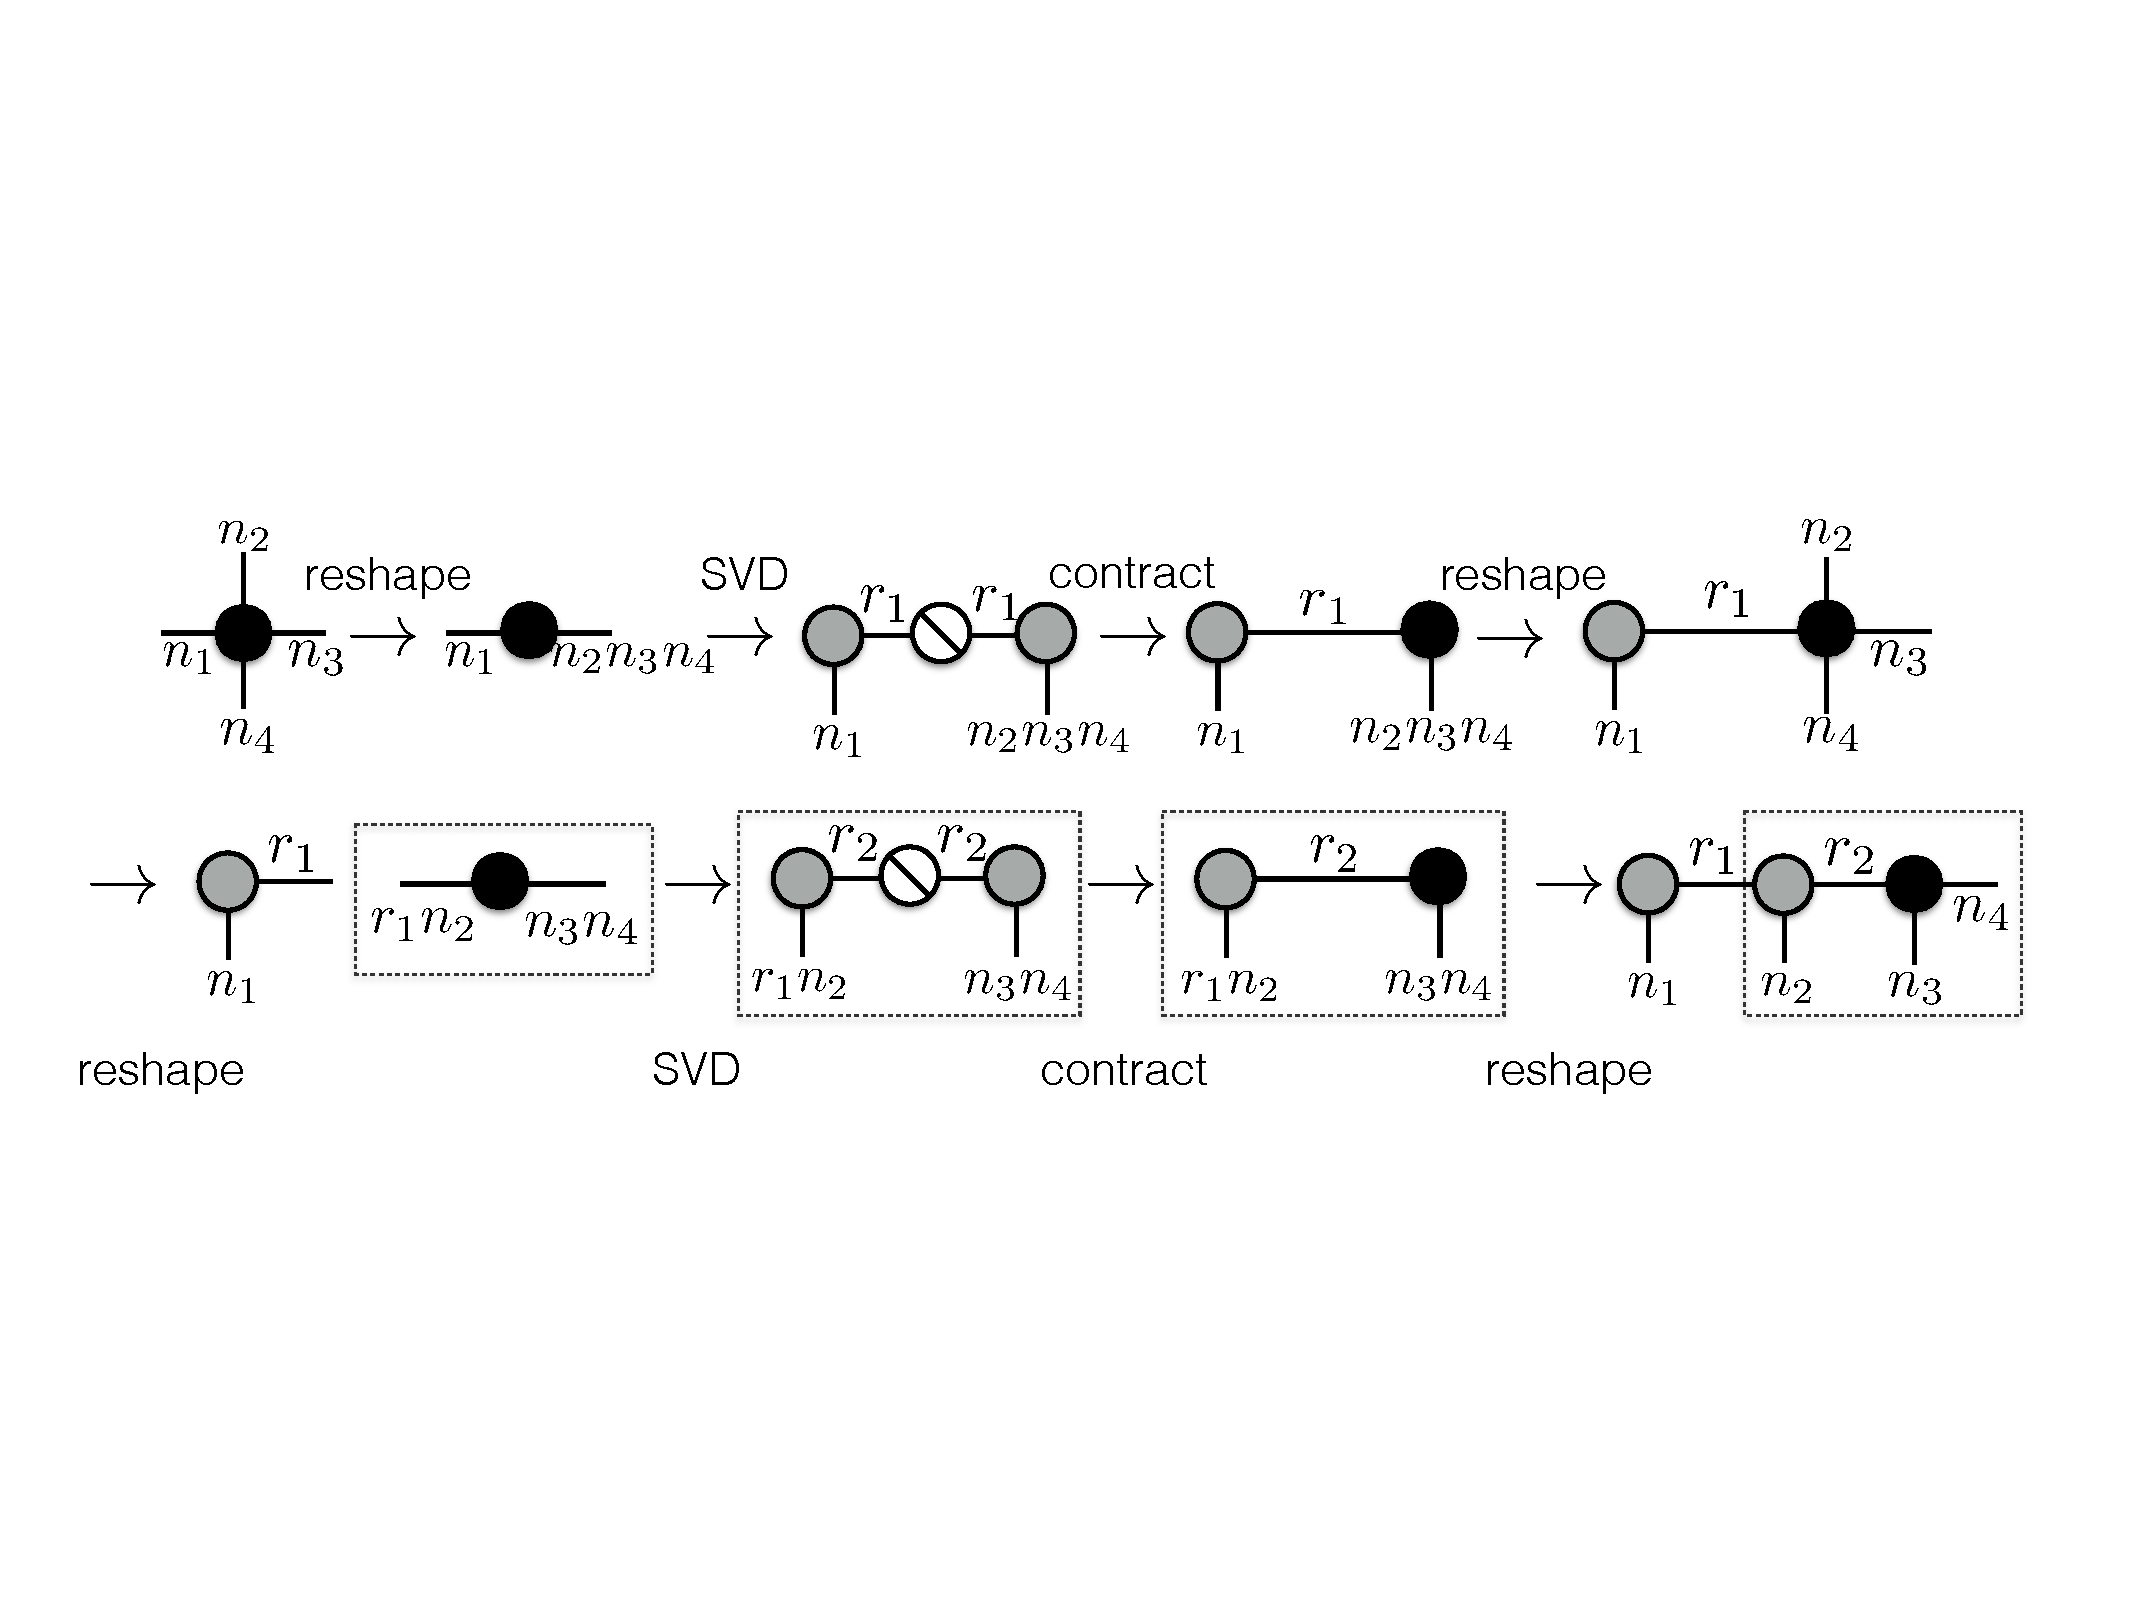
\includegraphics[width=\linewidth]{thpropfigs/ttsequence}
  \caption{The creation of the first two `carriages' of a tensor train decomposition for a 4-way tensor.}
  \label{fig:ttsequence}
\end{figure}

\paragraph{Proposal}
We summarize our proposed contributions as follows:
\begin{itemize}
  \item Implement the first distributed-memory implementation of the tensor train decomposition.
  \item Analyze the communication and computation behavior of the `reshape-SVD' method in distributed memory.
  \item Apply methods from our randomized Tucker decomposition to the tensor train in distributed memory.
  \item Benchmark both methods on a supercomputer and analyze/establish tradeoffs.
\end{itemize}

% \section{Streaming Graph Partitioning} \label{sec:graph}
% \input{05-graph}
%
% \section{Timeline}

\bibliographystyle{siamplain}
\bibliography{bib,newbibs,tensbib}

\end{document}
